\documentclass{article}
\usepackage{graphicx} % Required for inserting images
\usepackage{amsfonts}
\usepackage{amsmath}
\usepackage{amssymb}
\usepackage{amsthm}
\usepackage{mathtools}
\usepackage{mathdots}
\usepackage{suppose}
\usepackage{booktabs}
%\usepackage{venndiagram}
\usepackage{tikz}
\usetikzlibrary{arrows.meta, decorations.markings, positioning}
\usepackage{geometry}
%\usepackage[table,dvipsnames]{xcolor}
%\definecolor{LightGray}{gray}{0.9}
%\usepackage{multicol}
%\usepackage{color}
%\setlength{\columnseprule}{1pt}
%\def\columnseprulecolor{\color{black}}
\newcommand{\Or}{\text{ or }}
\newcommand{\AND}{\text{ and }}
\newcommand{\Say}{\text{Say }}
\newcommand{\Let}{\text{Let }}
\newcommand{\For}{\text{ for }}
\newcommand{\Forall}{\text{ for all }}
\newcommand{\On}{\text{ on }}
\newcommand{\Take}{\text{Take }}
\newcommand{\From}{\text{From }}
\newcommand{\Where}{\text{ where }}
\newcommand{\Note}{\textbf{Note: }}
\newcommand{\pl}{\left(}
\newcommand{\pr}{\right)}
\newcommand{\bl}{\left[}
\newcommand{\br}{\right]}
\newcommand{\Cl}{\left\{}
\newcommand{\Cr}{\right\}}
\newcommand{\mb}{\mathbb}
\newcommand{\mc}{\mathcal}
\newcommand{\Span}{\text{span}}
\newcommand{\Range}{\text{range}}
\newcommand{\Null}{\text{null}}
\newcommand{\Sin}[1]{\sin(#1)}
\newcommand{\Cos}[1]{\cos(#1)}
\newcommand{\response}{\subsubsection*{Response}}
\newcommand{\note}{\textbf{Note:\text{ }}}
\newcommand{\contra}{$\rightarrow\leftarrow$}
\newcommand{\resetal}{\setcounter{equation}{0}}
\usepackage{enumitem}
\newcommand{\nc}[1]{(#1)}
\setlist[enumerate,1]{label=\nc{\alph*}}
\setlist[enumerate,2]{label=\nc{\roman*}}
\setlist[enumerate,3]{label=\nc{\roman*}}
\setlist[enumerate,4]{label=\nc{\arabic*}}
\newcommand{\Space}{\text{ }}
\renewcommand{\labelitemi}{\textendash} 
\renewcommand{\labelitemii}{\textasteriskcentered} 
\renewcommand{\labelitemiii}{\textbullet} 
\renewcommand{\labelitemiv}{\textperiodcentered} 
%\usepackage{pgfplots}
%\pgfplotsset{compat=1.18}
%\usepackage{etoolbox}
%\usepackage{colortbl}
\usepackage{setspace}
\usepackage[indent=0.25in]{parskip}
\usepackage{bm}
\usepackage{nicematrix}
\usepackage{dirtytalk}
\usepackage{pdfpages}
\usepackage{logicproof}
\usepackage{etoolbox}
\usepackage{arydshln}
\makeatletter
\renewcommand{\lp@start@proof@line}{%
  \stepcounter{lp@line}%
  (\arabic{lp@line})%  
  &%
  \lp@continue@proof@line%
}
\makeatother
\usepackage{hyperref} 
\hypersetup{
      colorlinks=true,
      linkcolor=blue,
      citecolor=blue,
      urlcolor=blue
    }
\usepackage{mathrsfs}
\usepackage{algpseudocode}
%\newcommand{\Lapl}{\mathscr{L}}
%\newcommand{\iLapl}{\mathscr{L}^{-1}}
\renewcommand{\thesection}{Question \arabic{section}}
\renewcommand{\contentsname}{Table of Contents}
\renewcommand{\theequation}{\arabic{equation}}
\usepackage[backend=biber,
style=verbose,dashed=false]{biblatex}
\addbibresource{bib.bib}
\defbibheading{bibliography}[\bibname]{%
  \section*{\centering#1}%
}
\newcommand{\Ang}[1]{\left\langle #1 \right\rangle}
\urldef{\repourl}\url{https://github.com/14arjunk/CNET5051_Assignments/tree/main/Assignment%202%20Files}



\title{\textbf{Assignment 2}}
\author{Arjun G. Kumar\\
CNET 5051\\
Northeastern University}
\date{17 October 2026}

\begin{document}
\maketitle
\tableofcontents
\listoffigures
\section*{Question 0}
\textit{Include your code in a (well-documented, commented, clear) }\texttt{assignment02.ipynb}\textit{ file. Scores for the code-based questions below will be based on your written responses and code.}
\response
Public repo \href{https://github.com/14arjunk/CNET5051_Assignments/tree/main/Assignment%202%20Files}{here.}\footnote{\repourl}
\section{}
\textit{In this question we will work with degree-controlled random graph null models.}
\begin{enumerate}
    \item \textit{\textbf{The Configuration Model.} First, implement the configuration model in Python. Your function should take a list of integers as a degree sequence, and return a graph where each vertex has the assigned degree. Your graph may contain duplicate edges and self-loops.}
    \item \textit{\textbf{The Chung Lu Model.} Next, implement the Chung Lu random graph model. Remember that this model creates an edge between nodes $i$ and $j$ with independent probabilities defined by vertex degree and the total number of edges in the graph:}
    \[
        p_{ij} = \frac{k_i k_j}{2m},
    \]
    \textit{where $2m \coloneqq \sum_i k_i$. Your implementation should take a list of integers as a degree sequence, and return a simple graph with approximately the desired degree sequence.}
    \item \textit{\textbf{Model Differences.} For the degree sequence }\texttt{degrees=[8,5,5,4,3,2,2,2,1,1,1,1,1,1,1]}\textit{, generate a thousand random graphs using the Configuration Model and the Chung Lu model, then:}
    \begin{enumerate}
        \item \textit{Plot the average adjacency matrix for each model. This should be a heatmap of:}
        \[
            \Ang{A} = \frac{1}{N}\sum_{i=1}^{N} A_i
        \]
        \textit{where $N$ is the number of generated random graphs, and $A_i$ is the adjacency matrix of the $i$th graph. (Hint: matplotlib's }\texttt{imshow}\textit{ is useful for displaying matrix data.)}
        \item \textit{Choose two graph metrics: one that should be approximately the same across graphs generated by both models, and one that should diverge significantly between the two models. For each metric, make a plot (histogram, kernel-density estimate, or cumulative distribution function) showing the distribution of the metric across all generated graphs from each model.}
    \end{enumerate}
    \textit{\textbf{Note:} For this stage you may remove self-loops and duplicate edges from your configuration model graphs if it helps make a direct comparison to Chung Lu graphs.}
    \item \textit{\textbf{Discussion.} Discuss the above results briefly. Why do the models produce similar results under some metrics and different results under others?}
\end{enumerate}
\response
\begin{enumerate}
    \item See .ipynb
    \item See .ipynb
    \item See .ipynb and figures below.
    \begin{enumerate}
        \item See \autoref{fig:heatmaps}
        \begin{figure}[ht!]
            \centering
            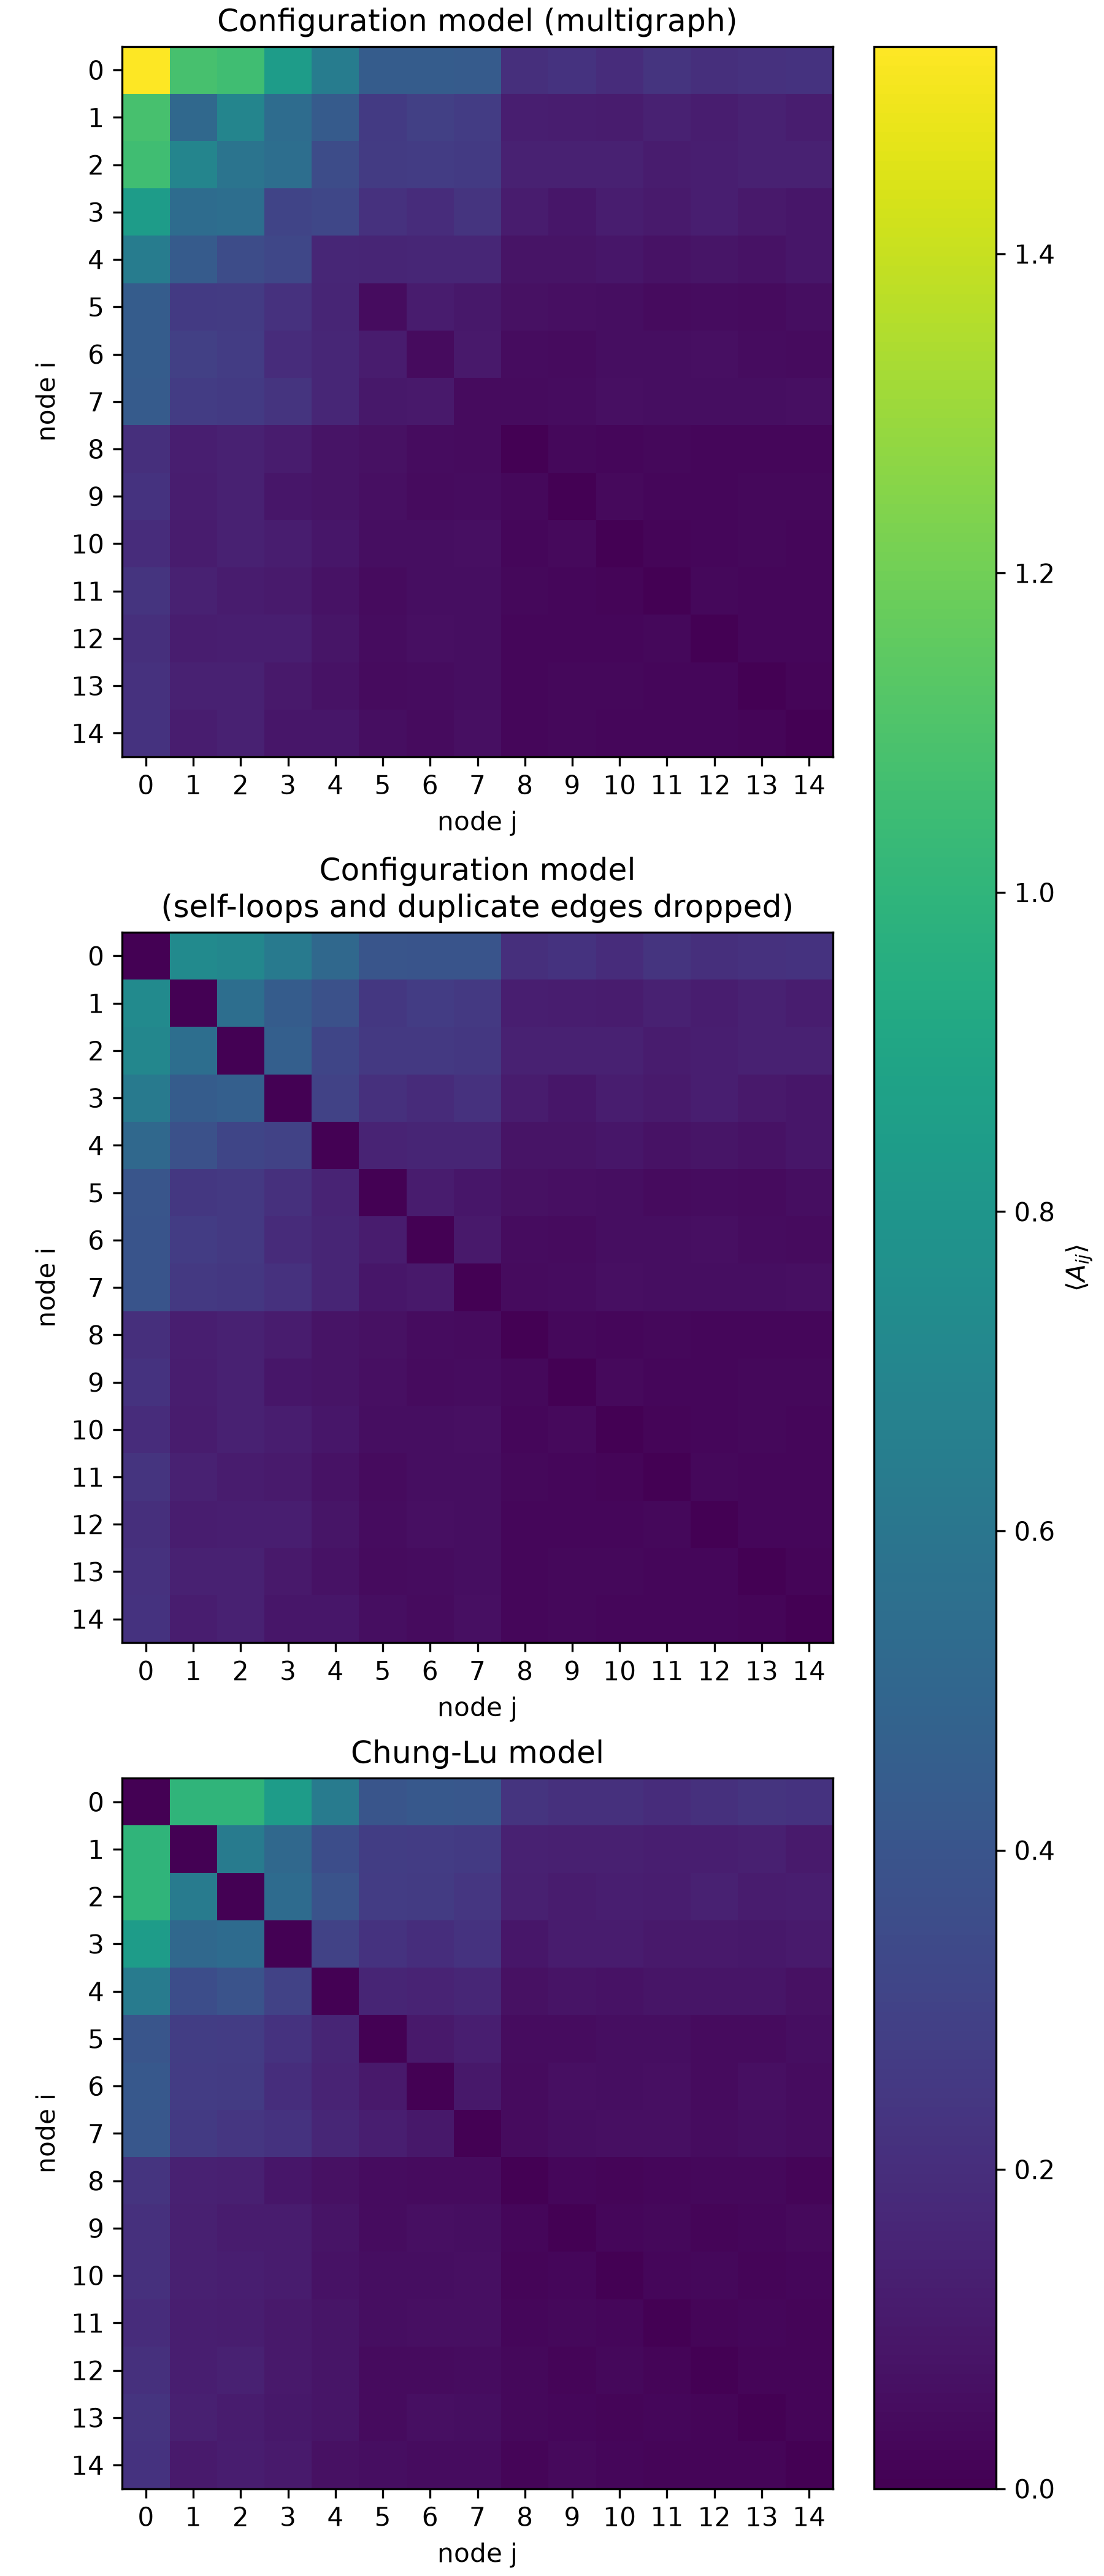
\includegraphics[width=0.65\linewidth]{Assignment 2 Files/configuration_chunglu_heatmaps.png}
            \caption{Comparative heatmaps of the CM, CM (Simple), and Chung-Lu}
            \label{fig:heatmaps}
        \end{figure}
        \item See \autoref{fig:isolated} and \autoref{fig:deg4}
        \begin{figure}[ht!]
            \centering
            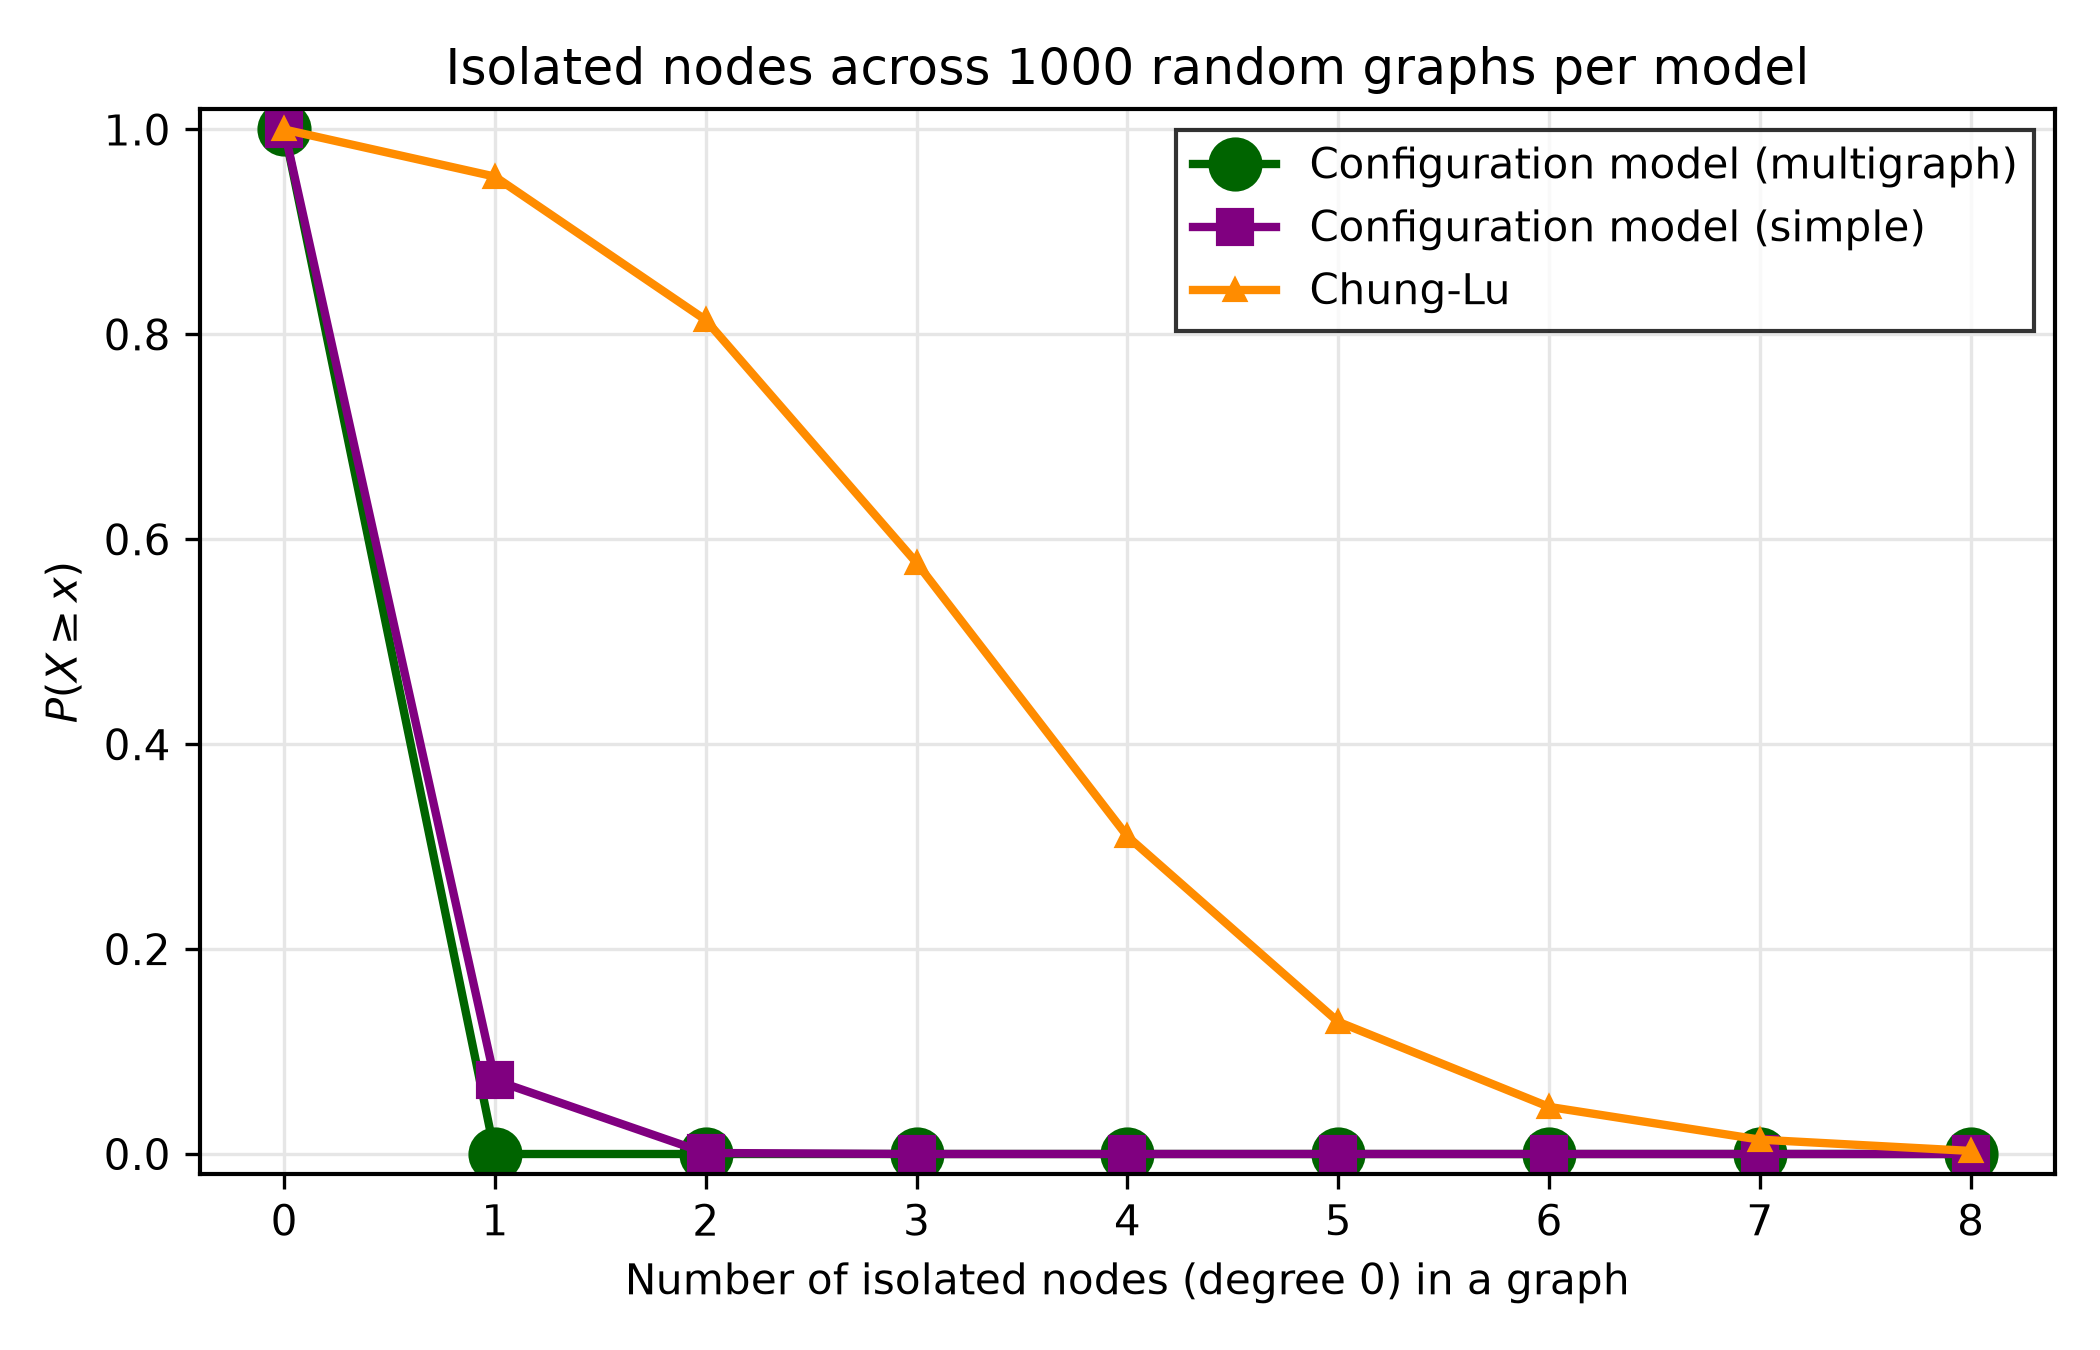
\includegraphics[width=0.85\linewidth]{Assignment 2 Files/isolated_nodes_ccdf.png}
            \caption{CCDFs of Nodes with $k=0$ for CM, CM (Simple), and Chung-Lu}
            \label{fig:isolated}
            \end{figure}
            \begin{figure}[ht!]
            \centering
            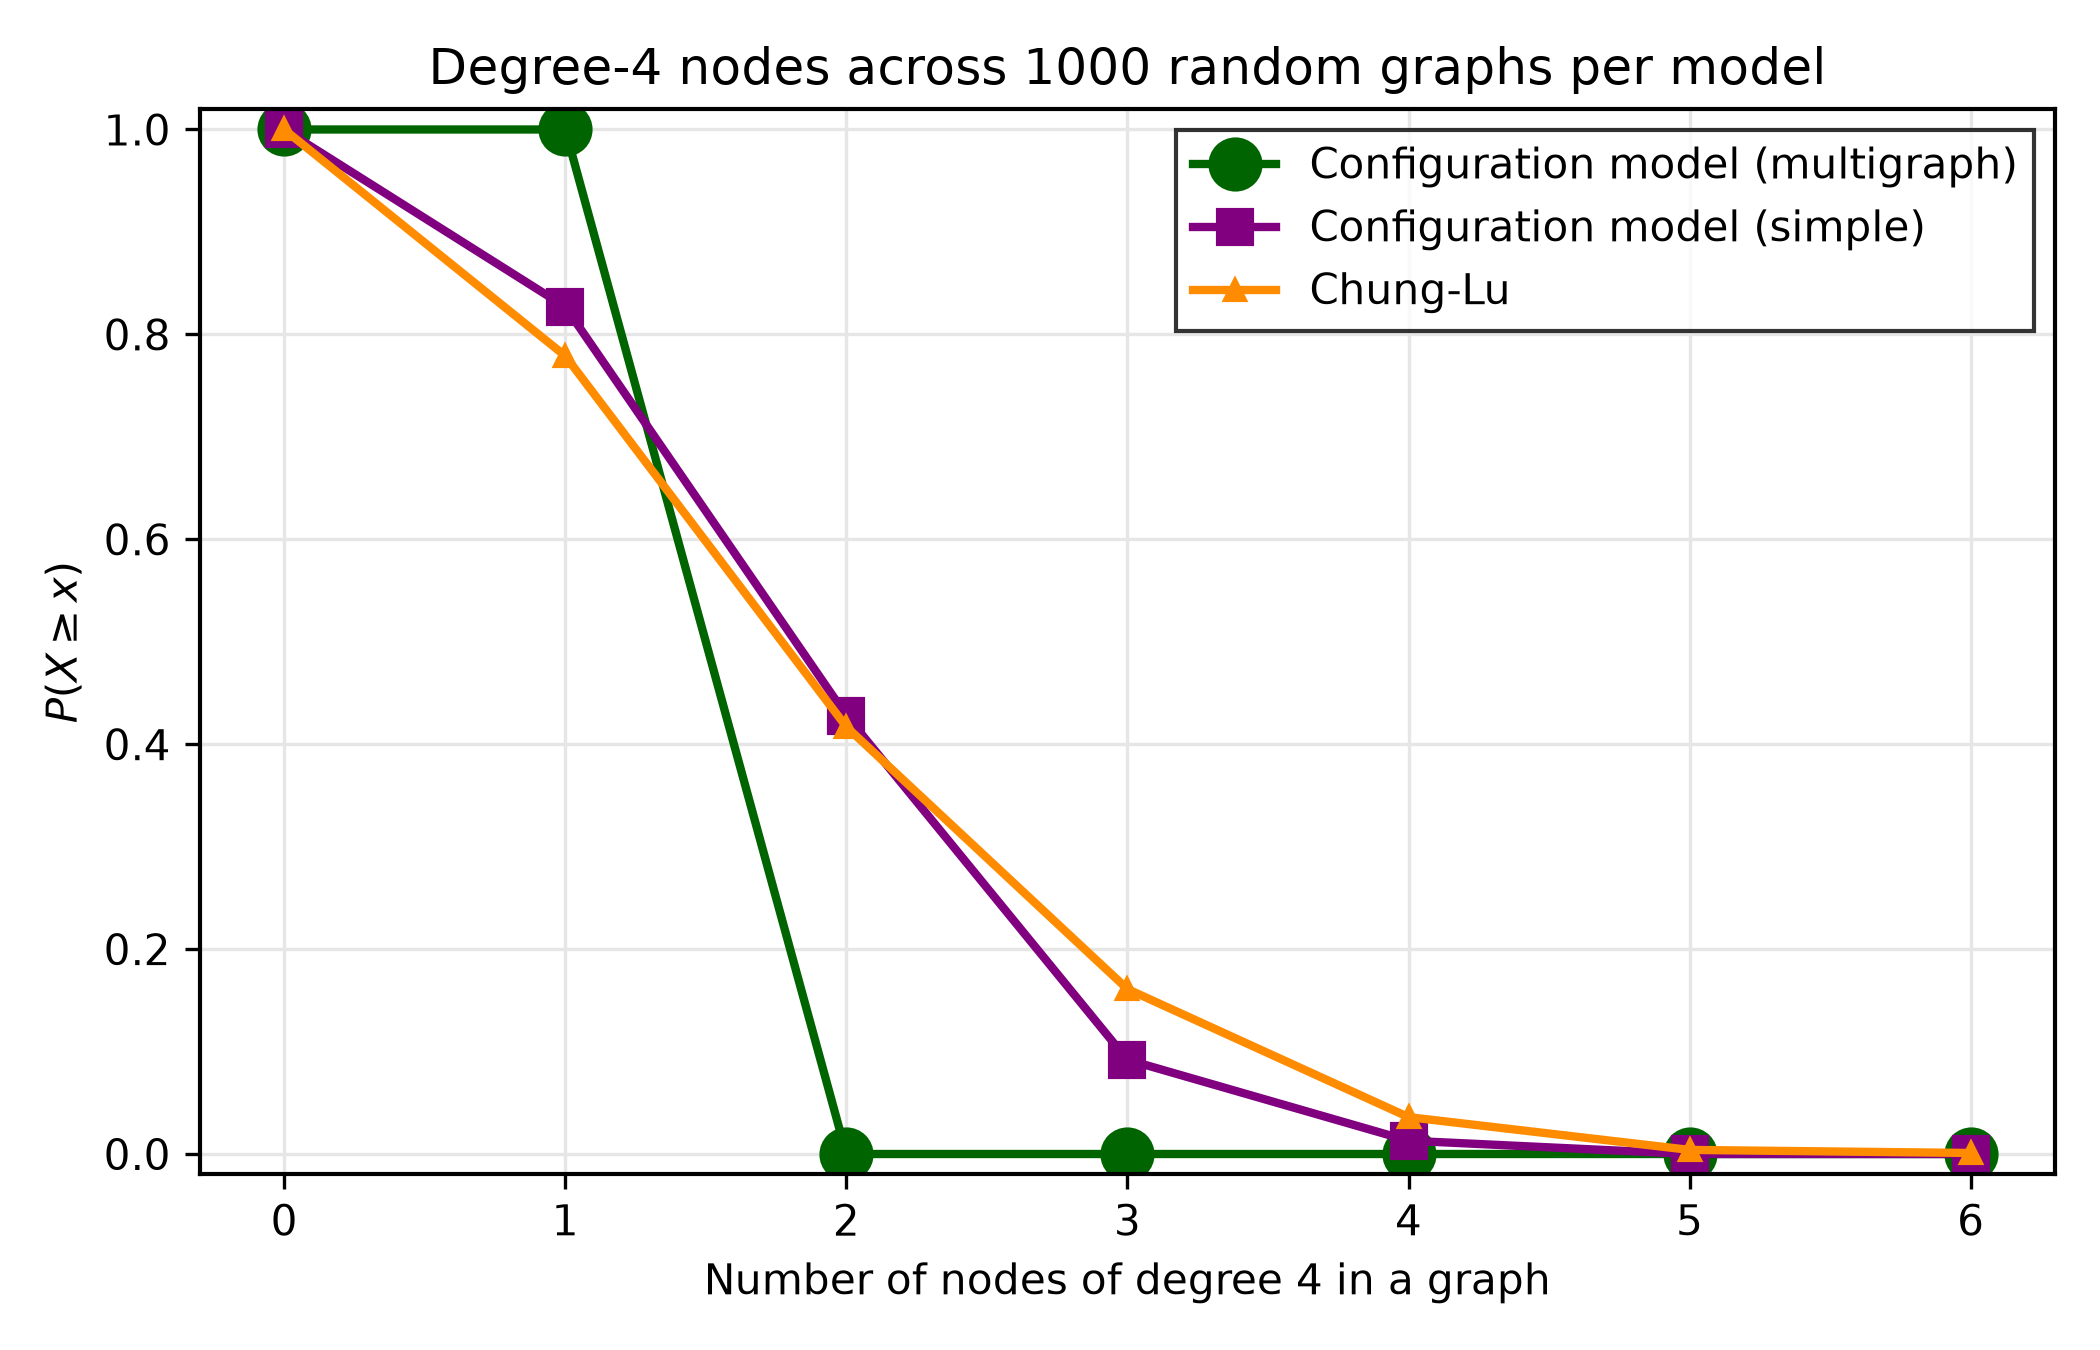
\includegraphics[width=0.85\linewidth]{Assignment 2 Files/degree4_nodes_ccdf.png}
            \caption{CCDFs of Nodes with $k=4$ for CM, CM (Simple), and Chung-Lu}
            \label{fig:deg4}
            \end{figure}
    \end{enumerate}
    \item \autoref{fig:heatmaps} contains 3 panels which are the heatmaps of $\langle A \rangle$ for each model: Configuration Model, Configuration Model (Simple), and Chung-Lu. The nodes are sorted by target degree in the degree sequence, so $k_0=8$ and $k_8,\dots,k_{14}=1$. All panels share the same color scale for readability. 

This helps us to assess if all three models are producing ``similar" graphs. 
\begin{itemize}
    \item We are seeing a similar overall pattern in all 3. The brighter blocks to the top left (hub-to-hub pairs) paired with fading to dark in the bottom right (leaves). All models are pairing nodes $i,j$ in proportion to $k_i,k_j$, so high degree nodes frequently connect to each other, and low degree nodes rarely do. 
    \item CM (multigraph) has a bright diagonal entry at $\langle A\rangle_{0,0}$ while Chung-Lu has none. Since self loops are permitted are only permitted in panel 1, we see the remaining diagonal entries form a 0 void across both CM (Simple) and Chung-Lu. 
    \item CM (multigraph) also has some entries off the diagonal with color indicating frequency above 1, due to the presence of parallel edges. 
    \item Chung-Lu collapses probabilities to 1 when they exceed it, guaranteeing the presence of certain edges, for example, $p_{0,1}=1$. In CM (simple), while that edge is frequently present, they are not always, accounting for the differences in panels 2 and 3. 
    \item On average, the models largely agree except at the hubs themselves, where CM (multigraph) and Chung-Lu's capped probability each break expectations in a different way. In addition, the heatmaps only give means, and say nothing with regard to the variance of degree. For example, in CM (multigraph) every leaf has a degree of 1, whereas in Chung-Lu, some leaves end up as isolated nodes. 
\end{itemize}
\autoref{fig:isolated} and \autoref{fig:deg4} point out a simple metric (indicidence of nodes with a specified degree), one of which diverges and one of which is roughly similar. 

We expect the number of nodes with degree 0 to diverge because the CM (multigraph) fixes every node's degree exactly, so nobody in this degree sequence (all degrees $\geq 1$) can end up isolated. Rarely, in CM (simple) a degree-2 node can pair its two stubs together into a self-loop that we then delete. Chung-Lu only matches degrees in expectation. Seven of the 15 nodes have degree 1, we expect to see them have no edge at all with a significant probability, so we should see a few isolated nodes in a typical Chung-Lu graph, which matches the plot. 

We expect the number nodes with degree 4 to be broadly similar (around 1). In CM (multigraph), we always have exactly 1. In CM (simple) and Chung-Lu, some expected degree 3 nodes slide up to 4, and some expected degree 5 nodes slide down to 4, just as the single expected degree 4 node can also slide up or down. Overall, we see a rough balancing of around 80\% of realizations contain exactly 1 node of degree 4. 


\end{enumerate}
\clearpage
\section{}
\textit{In this question we will gain experience with community detection.}
\begin{enumerate}
    \item \textit{\textbf{Finding communities.} Download a network dataset from \url{https://networkrepository.com/} with between roughly $1{,}000 < N < 5{,}000$ nodes (select a different dataset from the one you used in assignment 1). Select a modularity maximization algorithm to detect communities in this graph.}
    \begin{enumerate}
        \item \textit{Visualize your network, coloring the nodes by community membership.}
        \item \textit{Report the modularity of the partition your algorithm found.}
        \item \textit{Report the number of communities detected.}
        \item \textit{Store your partition as a dictionary in the form of }\texttt{\{node\_id: community\_id\}}\textit{.}
    \end{enumerate}
    \item \textit{\textbf{Null models.} Create a degree-preserving randomization of your network, and run the community detection algorithm you chose in part a on your randomized graph. Store each partition as a dictionary in the form of }\texttt{\{node\_id: community\_id\}}\textit{.}
    \item \textit{\textbf{Plotting a null model comparison.} You should now have two dictionaries, corresponding to the partitions from parts a and b. Create a figure with two subplots: In each, plot the community size distribution of each partition. Your figure should be publication-quality, with well-labeled, consistent axes, log-scaled wherever relevant, etc.}
    \item \textit{\textbf{Analysis.} For the different partitions computed above, discuss how you would approach comparing this functions quantitatively. For example, imagine a function $f(p_1, p_2)$ that takes partitions $p_1$ and $p_2$ as input and returns a number corresponding to how similar or dissimilar the partitions are. What properties should this function $f$ have? For this question, base your answer on a technique used in the literature, after a brief search about methods for quantifying differences between graph partitions. You do not need to implement the function, a high-level discussion is sufficient.}
\end{enumerate}
\response
I have chosen to use this netwook with $N=1005$ nodes from SNAP (Stanford Network Analysis Project -- Large Network Dataset Collection) which tracks emails between members of a European research institute.\footcite{snap-email-eu-core,snapnets} I chose it because it actually has ground truth communities originating from the department of each of the researchers. It is a digraph and the nodes are given a numeric attribute corresponding to their home department at the institute. SNAP's site cites 2 papers\footcite{yin2017local,leskovec2007evolution}
for the data, in addition to the generic requested SNAP citations.

\begin{enumerate}
    \item See .ipynb for comments on data and various visualization attempts. 
    \begin{enumerate}
        \item The best visualization is in \autoref{fig:communitiesheatmap}. The nodes are sized as the size of the department in reality, with the largest portion of the pie chart being the community that department's members most often were classified into. The heatmap shows the \% of each department who was placed into each detected community (columns).
    \begin{figure}[ht!]
        \centering
        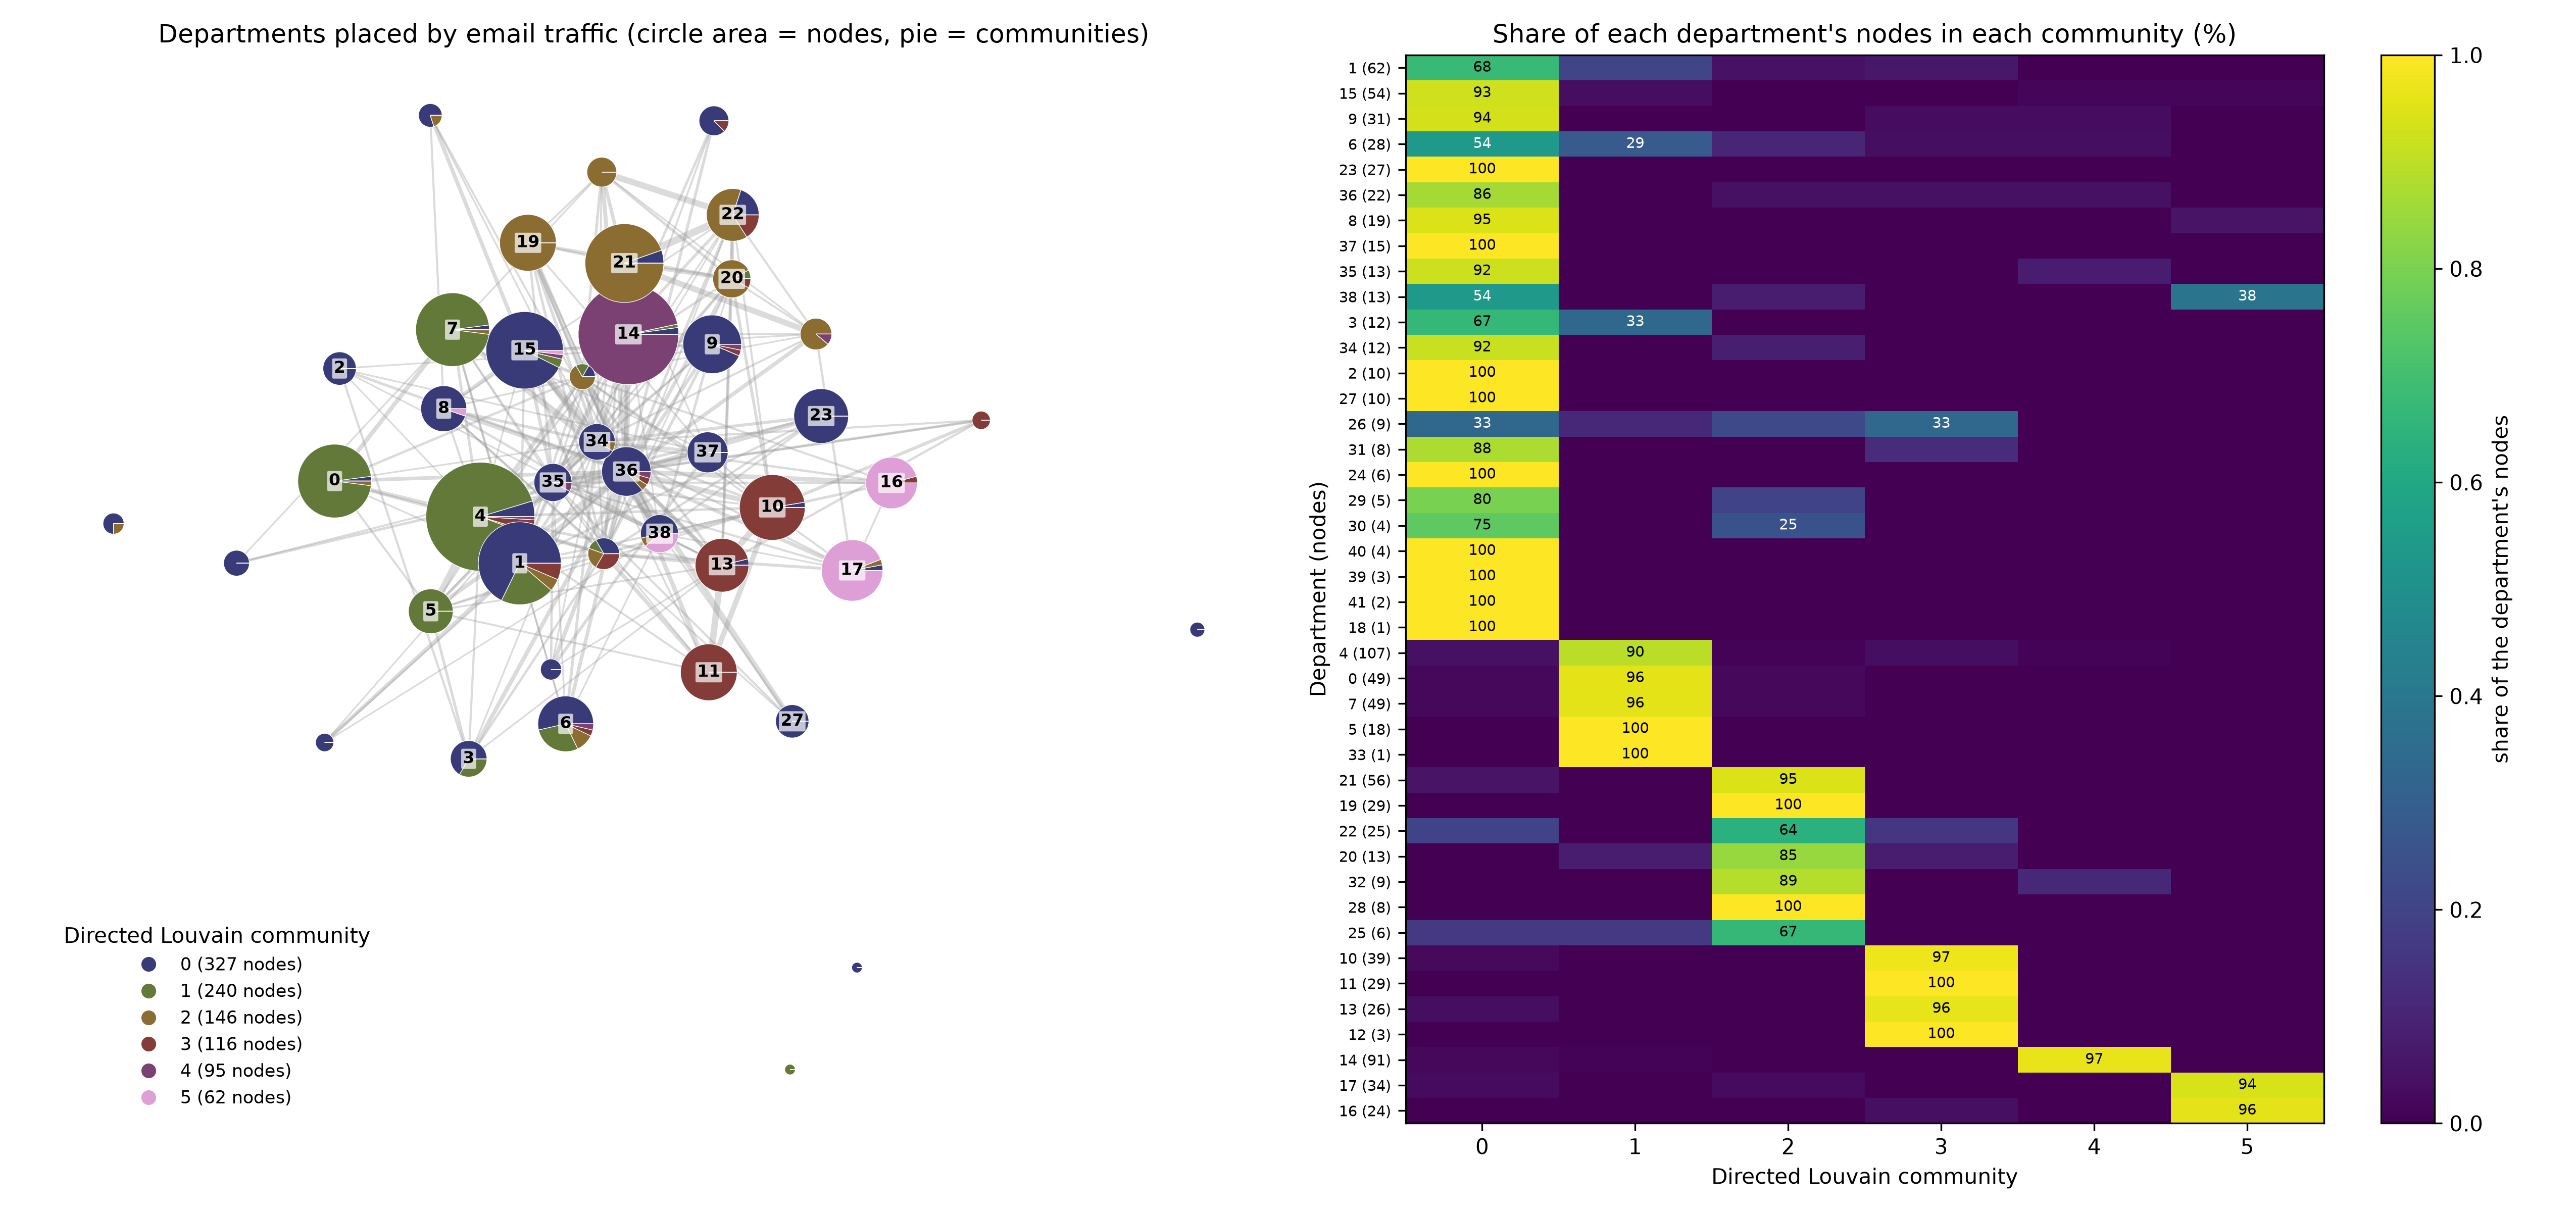
\includegraphics[width=1.1\linewidth]{Assignment 2 Files/email_departments_vs_communities.png}
        \caption{Communities found on directed EU research email network vs. department}
        \label{fig:communitiesheatmap}
    \end{figure}
    \item The modularity of the directed Louvain averaged 0.427 over 20 runs, with a minimum of 0.420 and a max of 0.429. 
    \item The directed louvain found 6 communities in this run. When run repeatedly, it averaged 7.5 with a min of 6 and a max of 8. 
    \item \texttt{partition\_dir} has stored the 6 communities.
    \end{enumerate}
    \item See .ipynb for the degree preserving directed edge swap null. The partition is stored in \texttt{partition\_null}.
    \item I think \autoref{fig:communitiesheatmap} is the cleanest visualization in order to understand the nature of the communities in this network, so \autoref{fig:randomcommunitiesheatmap} reproduces the style below with the randomized null. \autoref{fig:communitysizebars} plots the community size distributions. We can see a nearly flat distribution in the edge swapped null, compared to the steep slope of the original communities. The CCDF in \autoref{fig:communitysizeccdf} underscores this difference. 
    \begin{figure}[ht!]
        \centering
        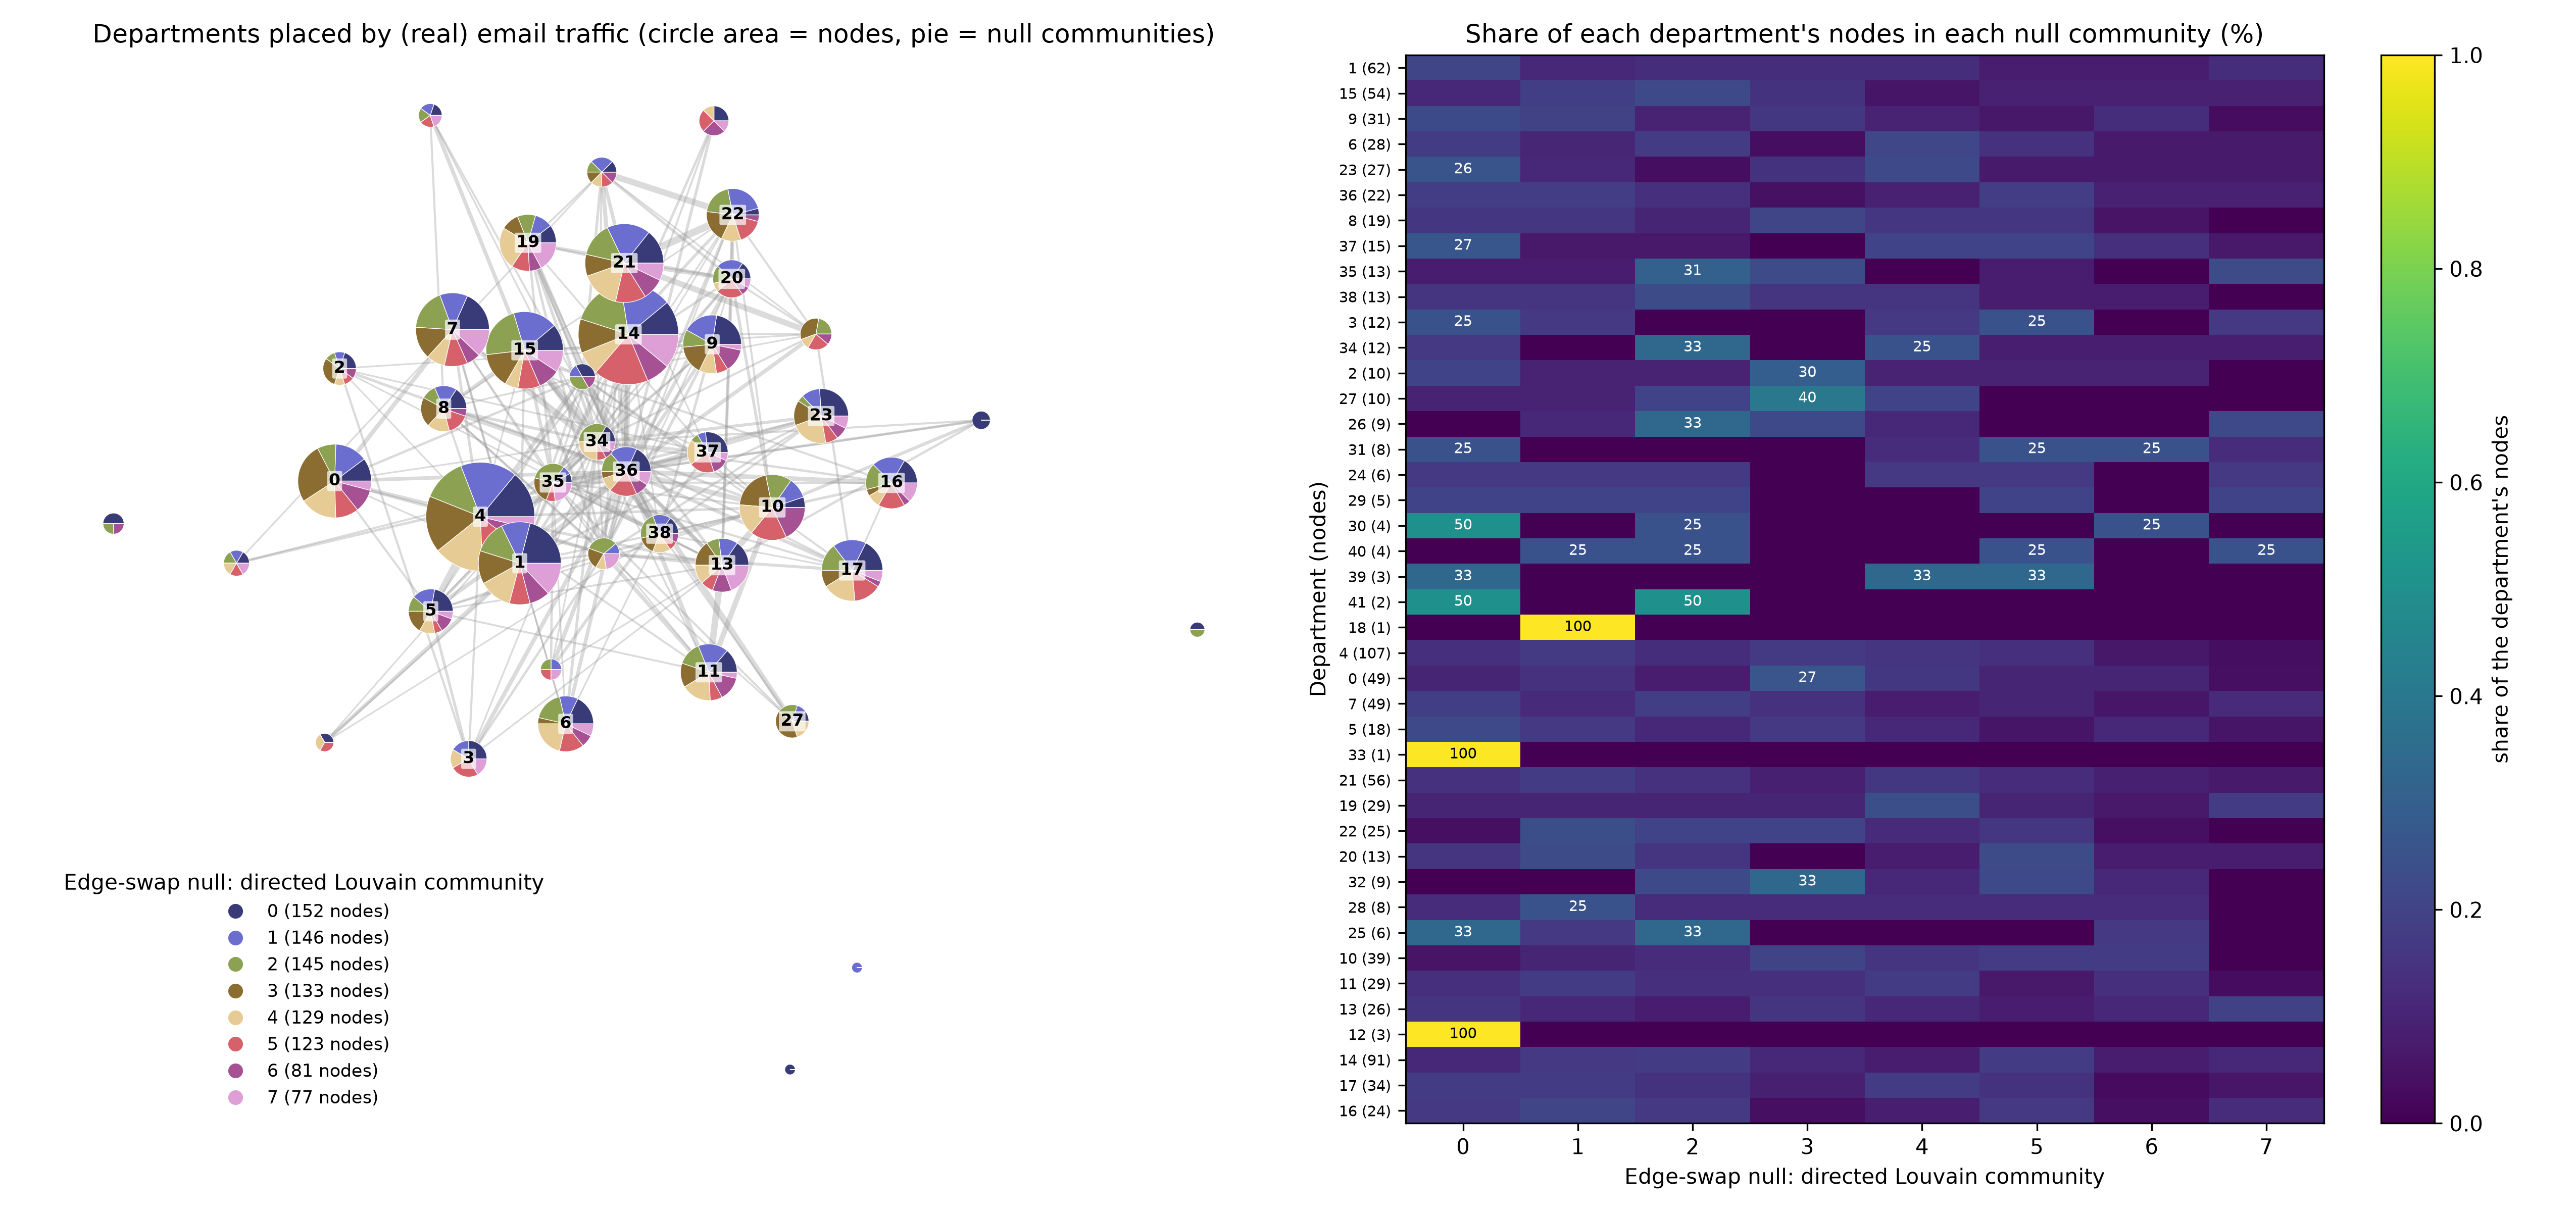
\includegraphics[width=1.1\linewidth]{Assignment 2 Files/email_departments_vs_null_communities.png}
        \caption{Communities found on directed EU research email network vs. department after degree preserving edge swaps}
        \label{fig:randomcommunitiesheatmap}
    \end{figure}
    \begin{figure}[ht!]
        \centering
        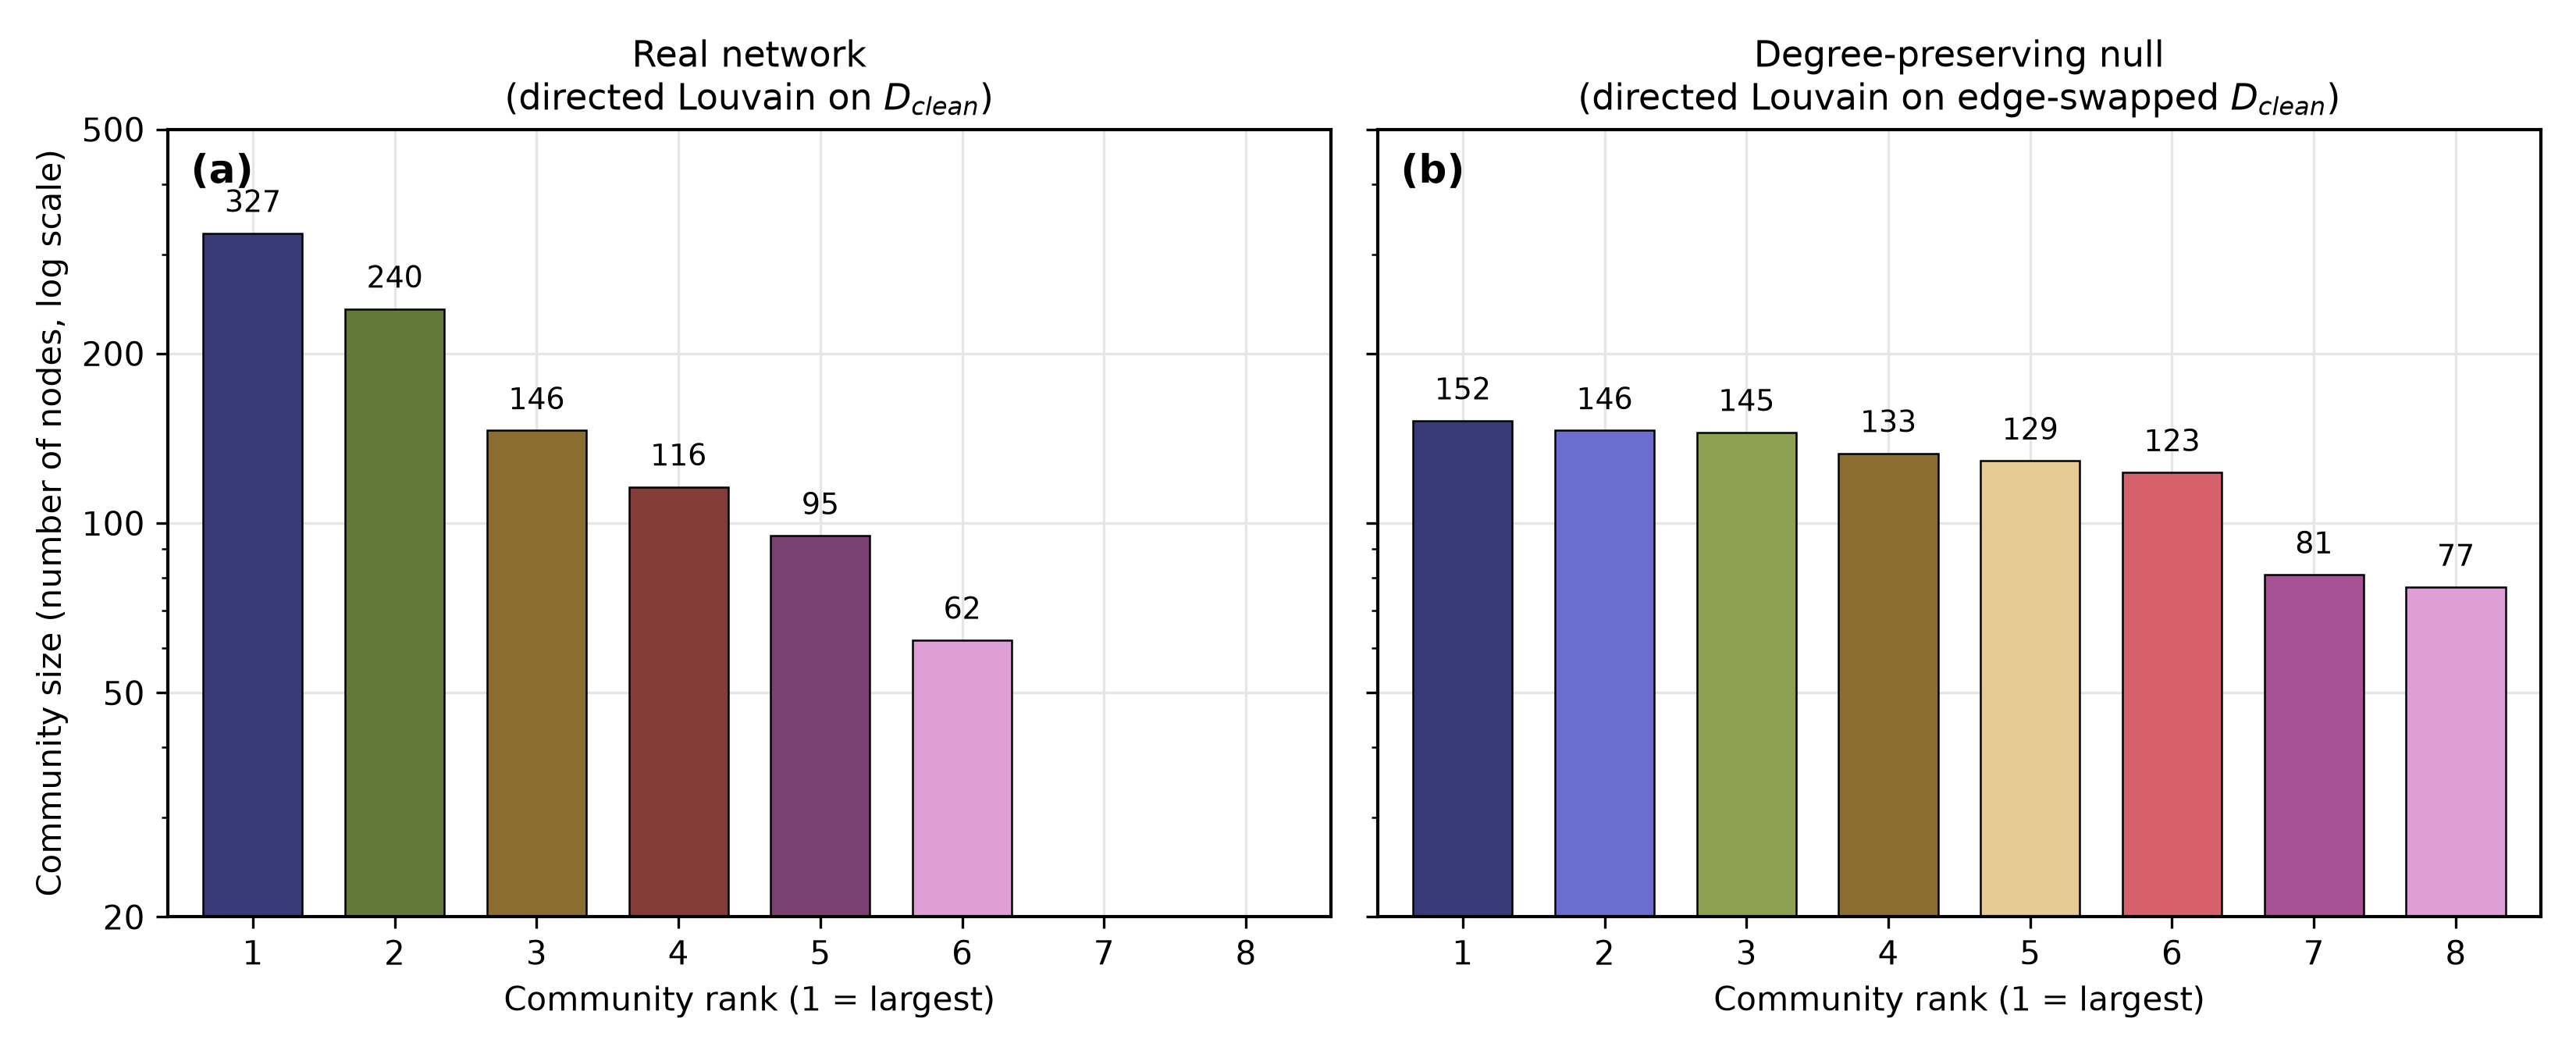
\includegraphics[width=1.1\linewidth]{Assignment 2 Files/community_size_distributions.png}
        \caption{Community size distributions in original EU email network vs. null}
        \label{fig:communitysizebars}
    \end{figure}
    \begin{figure}[ht!]
        \centering
        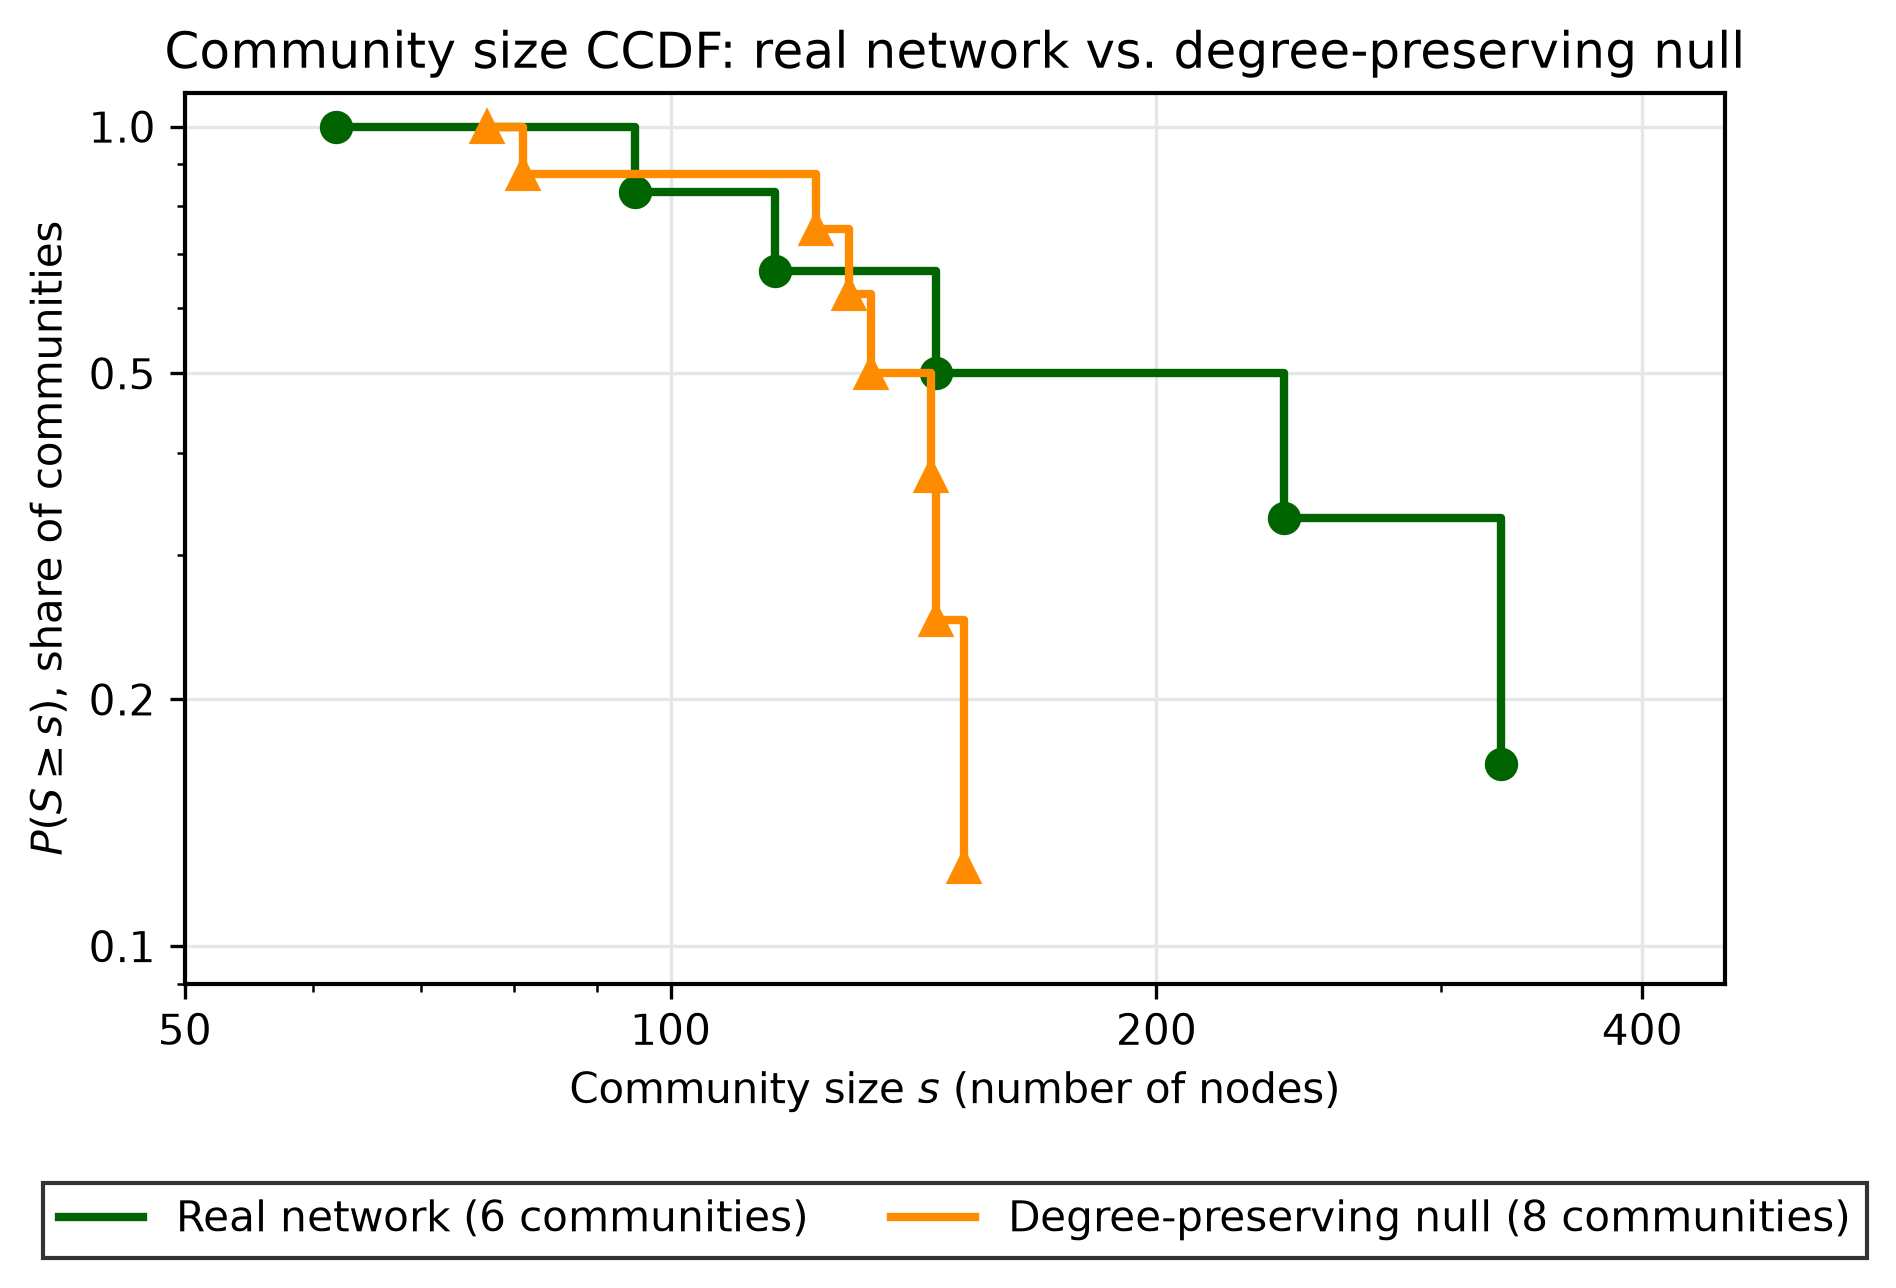
\includegraphics[width=1\linewidth]{Assignment 2 Files/community_size_ccdf.png}
        \caption{Distribution of community sizes in original EU email network vs. null}
        \label{fig:communitysizeccdf}
    \end{figure}
    \item When thinking about a useful $f(p_1,p_2)$ a few features immediately come to mind:
    \begin{enumerate}
        \item Different sized partitions: the function should be capable of comparing different numbers of communities (not merely check two different 6-partitions against one another).
        \clearpage
        \item Normalized appropriately: to compare communities of varying sizes (or indeed graphs of varying sizes creater naturally larger communities). 
        \item Merge vs. split: while perhaps less critical, when comparing against a known ground truth, a sensitivity (perhaps by sign) for "badness" stemming from which type of error is useful. Merging two real communities into one (as we are doing with the research departments), is a different error from splitting a true community. 
    \end{enumerate}

    After a brief literature search (Meila 2007, Danon et. al. 2005, Vinh et. al. 2010, Good \& Clauset 2010), I decided on variation of information (VI),\footcite{meila2007comparing} to compare two partitions $p_1$ and $p_2$ of the same nodes. This measures the information lost and gained in moving from one partition to the other:
\begin{equation}
    \mathrm{VI}(p_1,p_2) = H(p_1 \mid p_2) + H(p_2 \mid p_1) = H(p_1) + H(p_2) - 2\,I(p_1,p_2),
\end{equation}
where $$H(p) = -\sum_k \frac{n_k}{n}\log_2\frac{n_k}{n}$$ is the entropy of the community sizes and $I(p_1,p_2)$ is the mutual information of the joint distribution $P(k,k') = |C_k \cap C'_{k'}|/n$. This meets each of my desired features above. 
\begin{enumerate}
    \item It is built from the overlap table of the two partitions, so partitions with different numbers of communities pose no problem (for example 6 communities against 42 departments).
    \item It depends only on the relative community sizes $n_k/n$, so values are comparable across graphs of different sizes; it is not confined to $[0,1]$, but instead is bounded by $\log_2 n$ and and by $2\log K^*$ if both partitions have at most $K^*$ communities. We can normalize by $\log_2n$ if we want a $[0,1]$ metric, at the cost of comparing graphs of different $n.$
    \item Finally, when $p_1$ is a known ground truth $T$ and $p_2$ is the detected partition $C$, the two terms separate the two error types:
\begin{equation}
    \mathrm{VI}(T,C) = \underbrace{H(T \mid C)}_{\text{merging}} + \underbrace{H(C \mid T)}_{\text{splitting}},
\end{equation}
since $H(T \mid C)$ is large when a community mixes several true departments, and $H(C \mid T)$ is large when a department is spread over several communities.

This is a brief 10,000 foot survey of the method, and I'm sure I have not understood it deeply, nor properly elucidated its weaknesses, but at the moment it appears to be well-suited. 
\end{enumerate}

\end{enumerate}

\clearpage
\section{}
\textit{In this question we will revisit degree sequences with a focus on preferential attachment.}

\textit{We have worked with $G(n,p)$ random graphs extensively. We have also discussed how most graphs are not random, but follow some kind of preference for homophily or highly ``desirable'' nodes. One common preference is to connect to high degree nodes, reinforcing a rich-get-richer dynamic. We will create a network growth model, where we add new vertices to a graph, and create edges to existing vertices with a probability based on vertex $i$'s degree $k_i$:}
\[
    p(i) = \frac{k_i^{\alpha} + 1}{\sum_{j=0}^{n} \pl k_j^{\alpha} + 1 \pr}
\]
\textit{The $\alpha$ parameter allows us to configure the model between a sublinear preference for high-degree nodes ($0 < \alpha < 1$), a linear preference ($\alpha = 1$), and a superlinear preference ($\alpha > 1$). The $+1$ in the above equation ensures some chance of connecting to any vertex, even if it initially has a degree of zero.}
\begin{enumerate}[label=(\roman*)]
    \item \textit{\textbf{Implement the generator.} Write a graph generating function }\texttt{preferentialGenerator(n, a)}\textit{ that returns a graph with $n$ vertices and $\alpha = a$.}
    \item \textit{\textbf{Degree analysis.} Generate graphs with 1,000 nodes and alpha values of 0.1, 1, and 2. Make a plot comparing the three degree distributions. You may use histograms, kernel-density estimates, or cumulative distribution functions. However, your plots should be easy to interpret: select number of bins or bin widths, log scale, or other attributes as needed to produce a high-quality figure.}
\end{enumerate}
\textit{We will now pivot to the random walk model of network generation. In this model, every time we add a vertex $i$ we add two edges. First, an edge to an existing random vertex $j$. Then, with probability $p$, we add an edge from $i$ to a random neighbor of $j$. Otherwise we instead add an edge to another random vertex in the graph.}
\begin{enumerate}[label=(\roman*), resume]
    \item \textit{\textbf{Implement the generator.} Write a graph generating function }\texttt{randomWalkGenerator(n, p)}\textit{ that returns a graph with $n$ vertices generated by random walks with probability $p$.}
    \item \textit{\textbf{Clustering analysis.} Generate graphs with 1,000 nodes and $p$ values of 0, 0.1, 0.5, and 0.9. Make a plot comparing the four clustering distributions. As in part (ii), make these plots easily interpretable.}
\end{enumerate}
\textit{And finally\ldots}
\begin{enumerate}[label=(\roman*), resume]
    \item \textit{\textbf{Interpretation.} Compare the graphs created by the two network growth models. What kind of structures do they produce? In what circumstances might we want to use }\texttt{preferentialGenerator}\textit{ as a null model, and when might the random walk model be a more appropriate null assumption?}
\end{enumerate}
\response
\begin{enumerate}[label=(\roman*)]
    \item See .ipynb. The graph starts from a single node, and each new node picks its target with weight $k_i^\alpha + 1$. I added an optional \texttt{m} argument (edges per new node, default 1) since the question doesn't fix it. With $m=1$ every graph is a tree with $n-1$ edges, which keeps the degree comparison straightforward. For $m>1$ the targets are drawn without replacement so the graph stays simple.
    \item See \autoref{fig:padegree}. To avoid reading too much into one realization, the degrees are pooled over 20 graphs per $\alpha$ (seeds $10,\dots,29$), and plotted as a CCDF on log-log axes so no binning choices are needed.
    \begin{figure}[ht!]
        \centering
        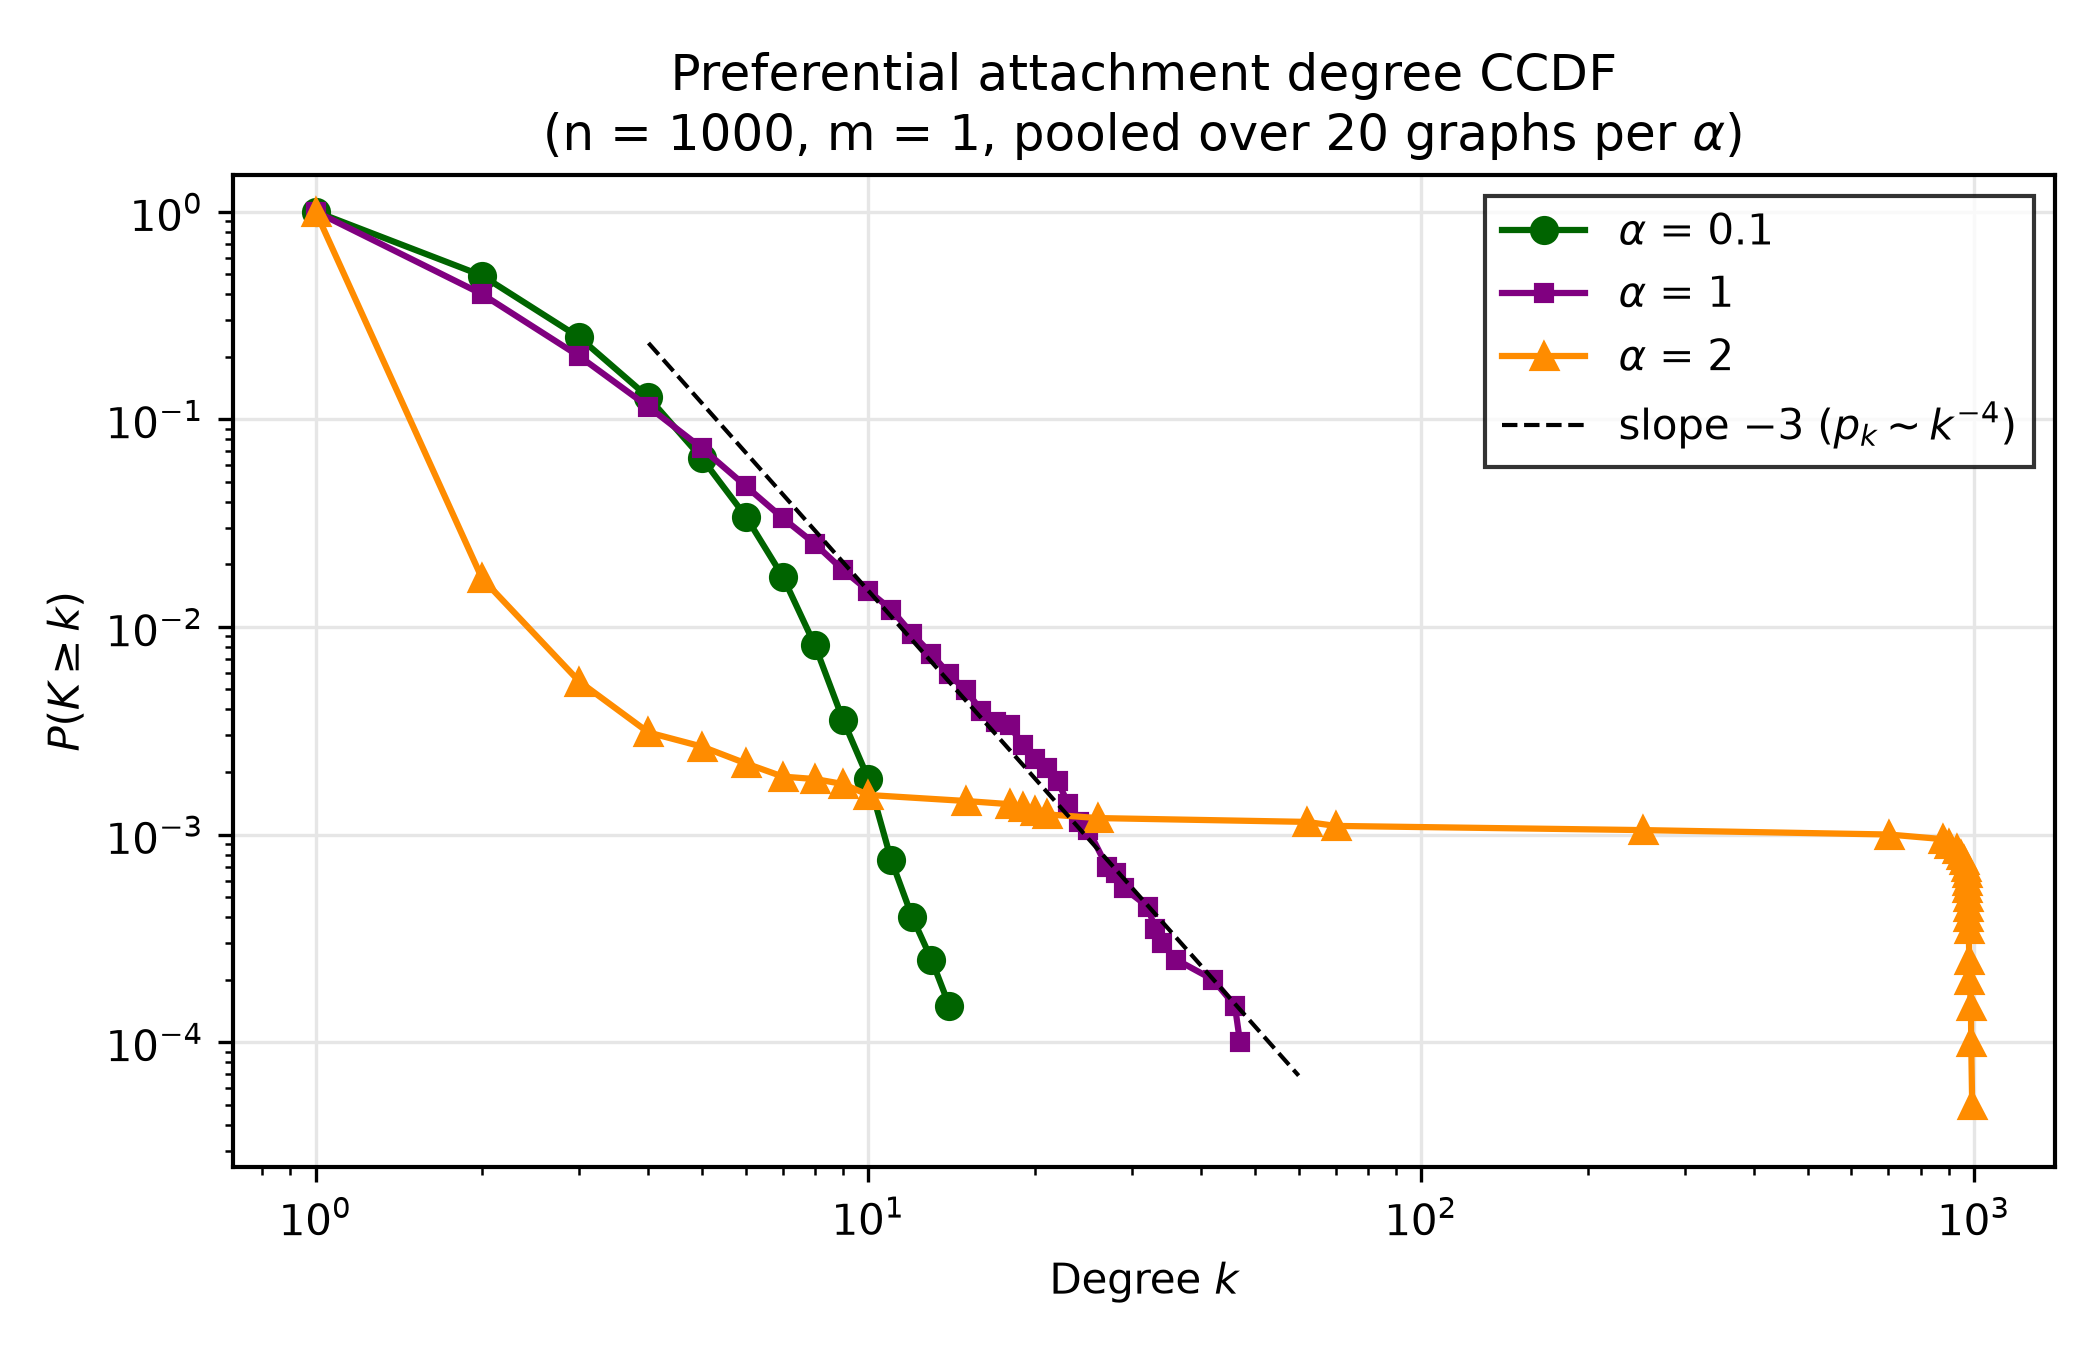
\includegraphics[width=0.85\linewidth]{Assignment 2 Files/preferential_degree_ccdf.png}
        \caption{Degree CCDFs of \texttt{preferentialGenerator} for $\alpha = 0.1, 1, 2$ ($n=1000$, $m=1$, 20 graphs each)}
        \label{fig:padegree}
    \end{figure}

    The three values of $\alpha$ land in the three regimes described by Krapivsky, Redner \& Leyvraz:\footcite{krapivsky2000connectivity}
    \begin{itemize}
        \item $\alpha = 0.1$ (sublinear): $k^{0.1}+1$ is nearly flat across the degree range, so every node is almost equally likely to be picked. The CCDF bends down quickly and is close to the $P(K \geq k) = 2^{-(k-1)}$ of a uniformly random tree (0.49, 0.25 and 0.13 at $k = 2, 3, 4$). No node passes degree 14 in any of the 20 graphs.
        \item $\alpha = 1$ (linear): this is Barab\'asi-Albert style preferential attachment,\footcite{barabasi1999emergence} and the tail is much heavier, reaching $k \approx 47$. Past $k \approx 10$ it is roughly parallel to the slope $-3$ guide. We expect this because with weight $k+1$ and $m=1$ a node's degree grows as $(k+1) \sim t^{1/3}$, which gives $p_k \sim k^{-4}$. The $+1$ makes the tail steeper than the classic $k^{-3}$. With $n = 1000$ the tail only covers about a decade of $k$, so I'd treat this as a consistency check rather than a fit.
        \item $\alpha = 2$ (superlinear): 98\% of nodes have degree 1, and the rest of the curve is essentially one hub per graph with $k \approx 950$ on average, i.e.\ about 95\% of all edges. Once one node is ahead, $k^2$ makes it so much more attractive that it captures nearly every new node, and the graph becomes a star. In a few graphs a second node got an early lead and kept some of its edges (the minimum hub share was 70\%), which is where the points around $k \approx 60$--$250$ come from.
    \end{itemize}
    \item See .ipynb. The graph starts from a triangle, so the first randomly chosen $j$ always has a neighbor to walk to. The neighbor of $j$ is chosen \textit{before} $i$ is attached, so the walk can't step back onto $i$. In the other case, the second node is drawn uniformly from every existing node except $j$. So the graph is always simple, with exactly $3 + 2(n-3)$ edges.
    \item See \autoref{fig:rwclustering}, again pooled over 20 graphs per $p$. Panel (a) is the CCDF of the local clustering coefficient $C_i$ (linear $x$ since $C \in [0,1]$, log $y$ since at $p = 0$ only about 5\% of nodes have any clustering at all). Panel (b) is the average clustering of the nodes of degree $k$, $C(k)$.
    \begin{figure}[ht!]
        \centering
        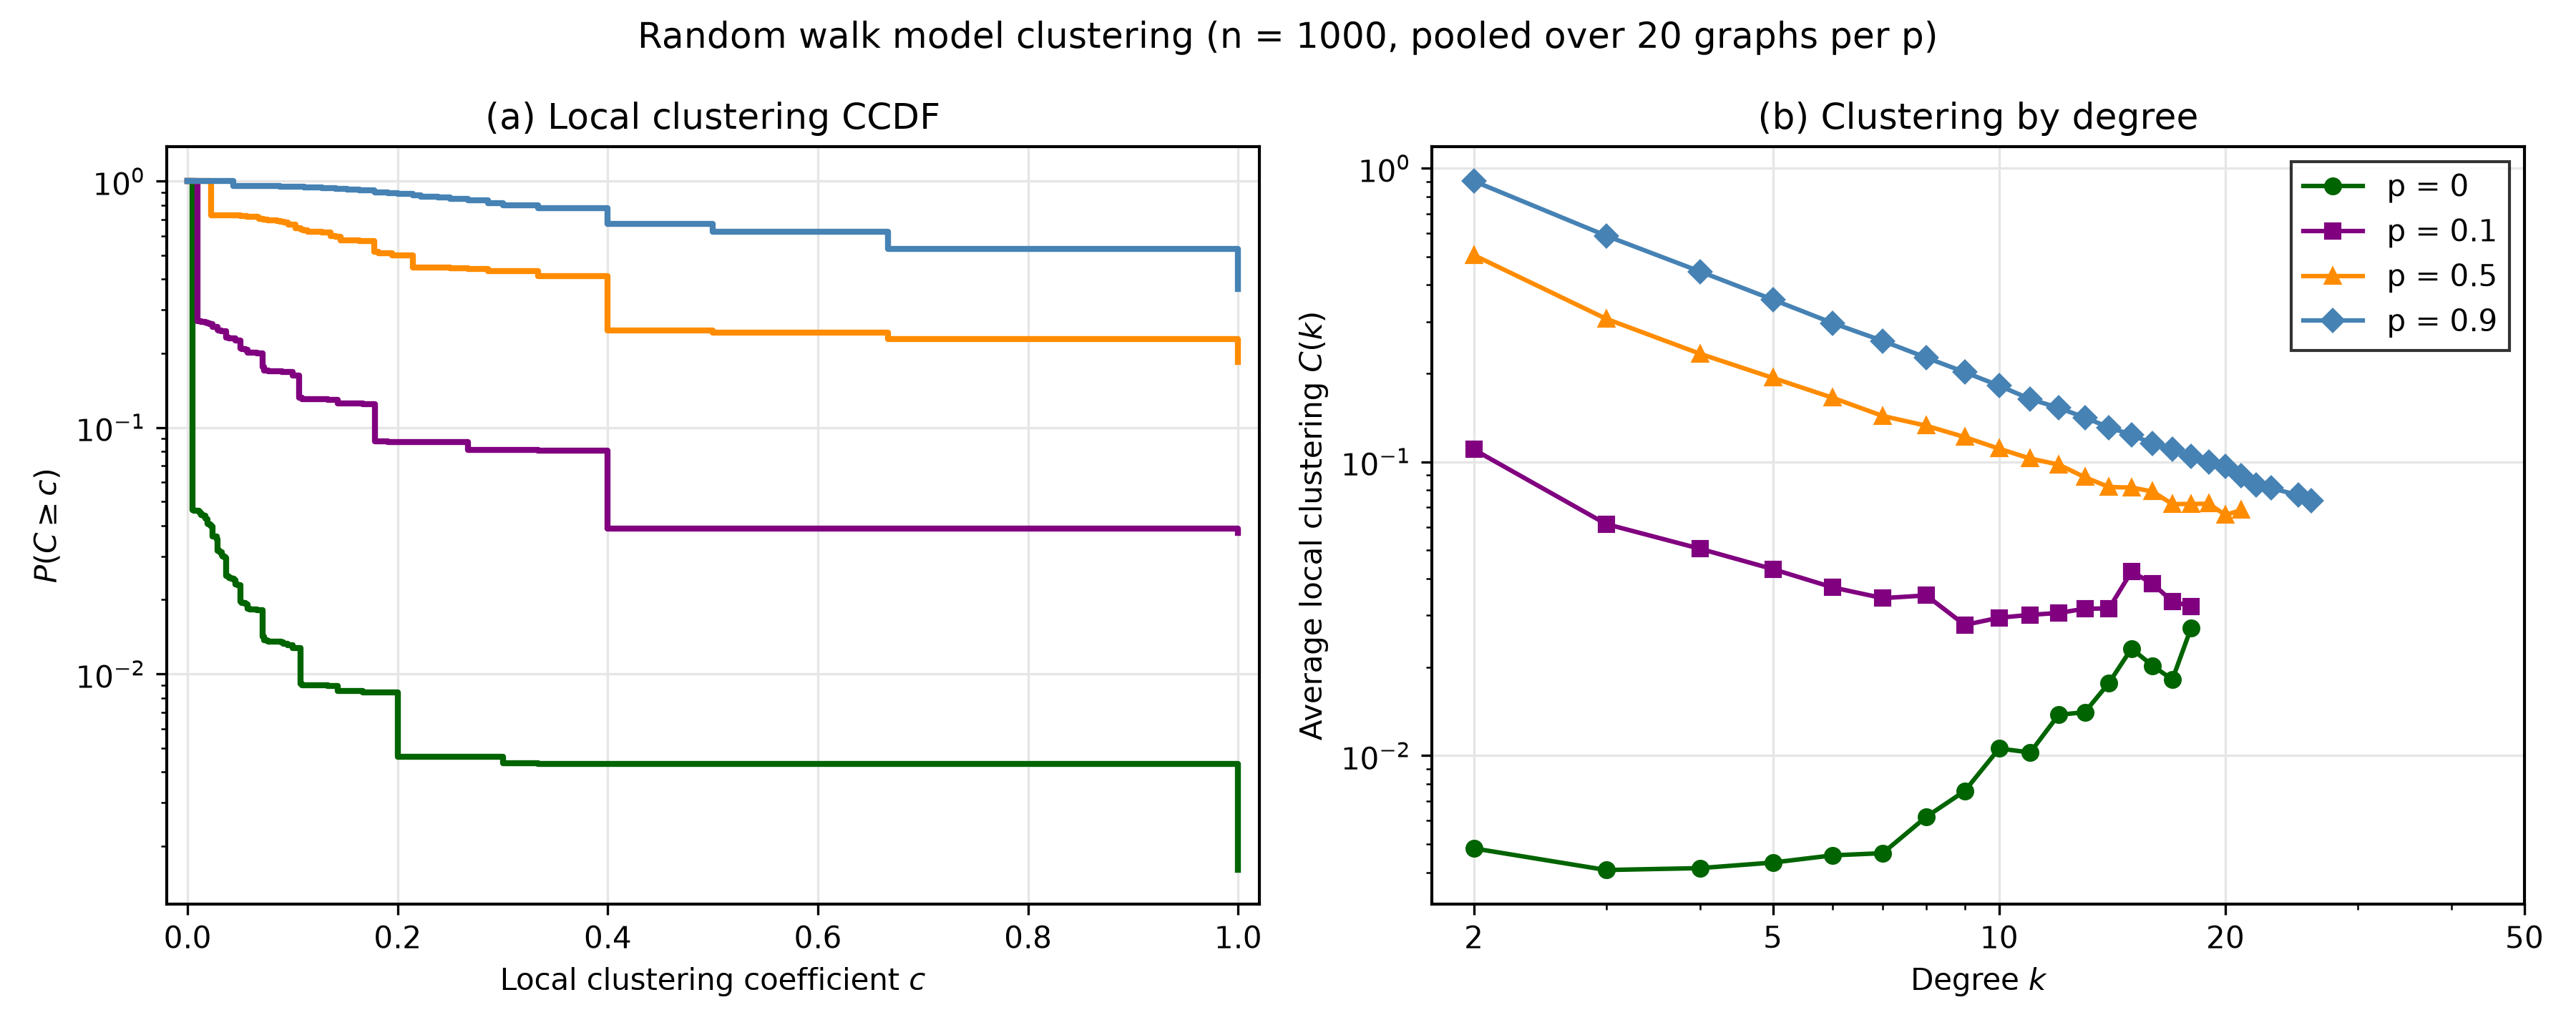
\includegraphics[width=1\linewidth]{Assignment 2 Files/random_walk_clustering.png}
        \caption{Local clustering of \texttt{randomWalkGenerator} for $p = 0, 0.1, 0.5, 0.9$ ($n=1000$, 20 graphs each)}
        \label{fig:rwclustering}
    \end{figure}

    Clustering rises steadily with $p$. The mean local clustering is 0.005, 0.069, 0.327 and 0.614, and the transitivity is 0.008, 0.041, 0.157 and 0.242, with very little spread across seeds.
    \begin{itemize}
        \item At $p = 0$ the second edge is uniformly random, so a triangle only forms by chance (when the two random targets happen to be neighbors), and almost every node has $C = 0$.
        \item Every node is born with degree 2, and a degree-2 node whose second edge went to a neighbor of $j$ sits in one triangle out of one possible, so $C = 1$ exactly. That is the value where each curve in (a) ends: at $p = 0.9$, 37\% of all nodes have $C=1$.
        \item In (b), for $p = 0.5$ and $0.9$, $C(k)$ falls off roughly as $1/k$ (a factor of 10 in $k$ costs about a factor of 10 in $C$). Each new node adds at most one triangle to $j$, while $\binom{k}{2}$ grows like $k^2$, so the hubs end up with low clustering. This is also why the transitivity, which weights high-degree nodes more, is well below the mean local clustering. At $p = 0$ the trend runs the other way, but those are chance triangles collecting among the oldest nodes, which have the most edges and are mostly connected to each other.
    \end{itemize}
    \item \autoref{tab:growthcompare} puts both models side by side on the same metrics (20 graphs each, $n = 1000$). It also includes preferential attachment with \texttt{m=2}, which adds the same two edges per node as the random walk model, so those rows have the same number of edges. \autoref{fig:rwdegree} compares their degree distributions.
    \begin{table}[ht!]
        \centering
        \small
        \begin{tabular}{lcccccc}
            \toprule
            Model & Edges & Max $k$ & Mean $C_i$ & Transitivity & Assortativity & Avg.\ path \\
            \midrule
            Preferential ($\alpha=1$, $m=1$) & 999 & 31.2 & 0.000 & 0.000 & $-0.083$ & 8.55 \\
            Preferential ($\alpha=1$, $m=2$) & 1997 & 58.6 & 0.016 & 0.010 & $-0.047$ & 4.31 \\
            Random walk ($p=0$) & 1997 & 18.6 & 0.005 & 0.008 & 0.134 & 4.94 \\
            Random walk ($p=0.1$) & 1997 & 19.3 & 0.069 & 0.041 & 0.122 & 4.99 \\
            Random walk ($p=0.5$) & 1997 & 24.4 & 0.327 & 0.157 & 0.087 & 5.25 \\
            Random walk ($p=0.9$) & 1997 & 33.8 & 0.614 & 0.242 & 0.032 & 5.84 \\
            \bottomrule
        \end{tabular}
        \caption{Preferential attachment vs.\ random walk model, means over 20 graphs with $n=1000$}
        \label{tab:growthcompare}
    \end{table}
    \begin{figure}[ht!]
        \centering
        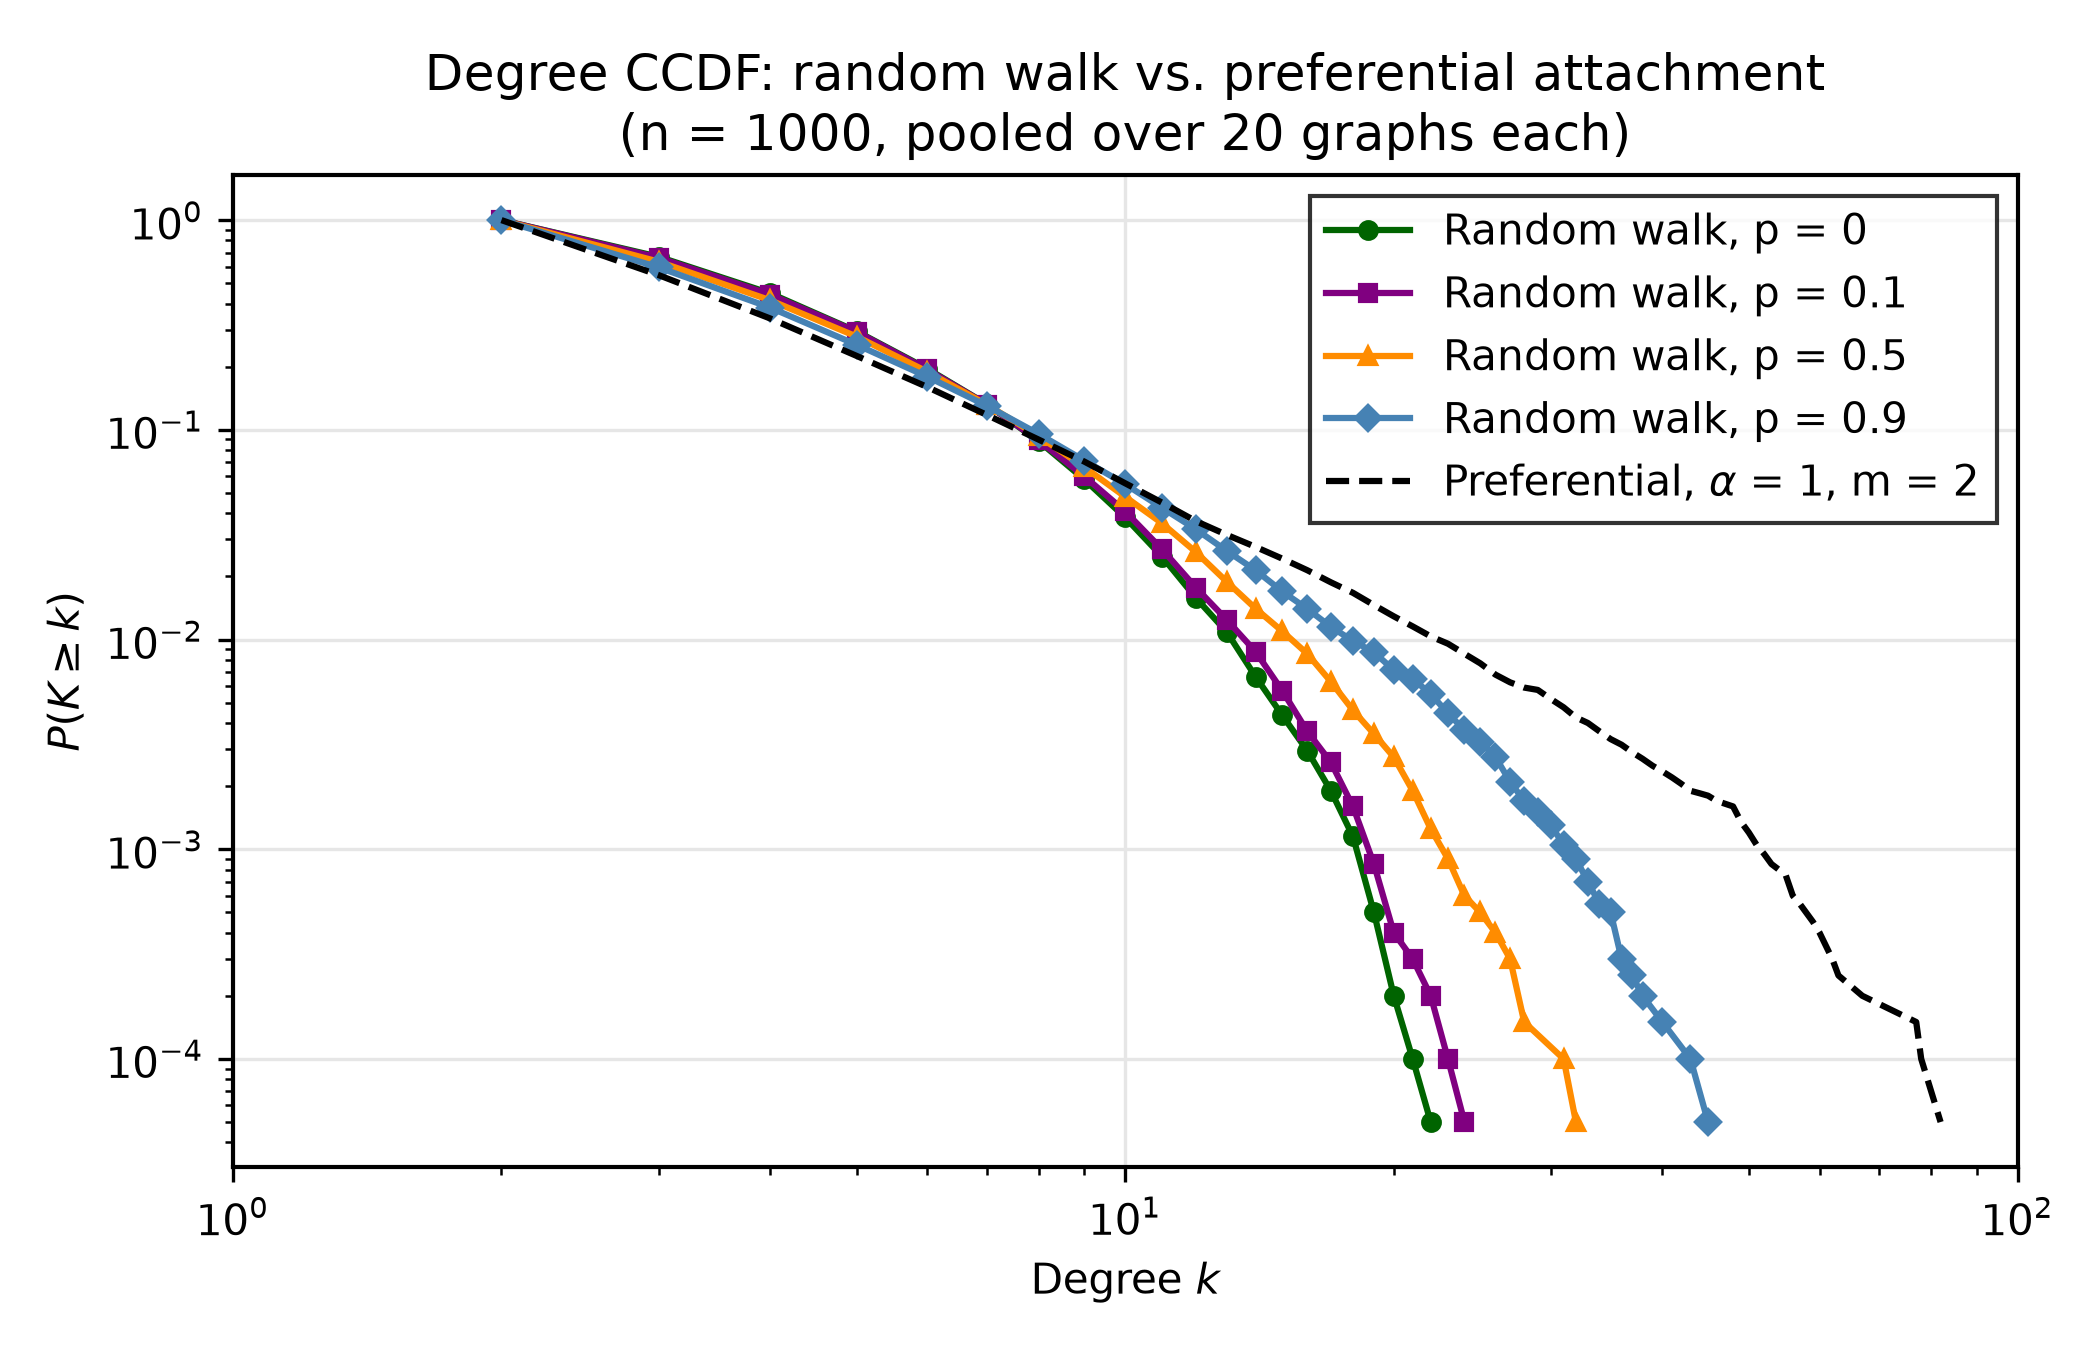
\includegraphics[width=0.85\linewidth]{Assignment 2 Files/random_walk_degree_ccdf.png}
        \caption{Degree CCDFs of the random walk model vs.\ preferential attachment with the same number of edges}
        \label{fig:rwdegree}
    \end{figure}

    The two models produce quite different structures:
    \begin{itemize}
        \item \texttt{preferentialGenerator} builds hubs and almost nothing else. With $\alpha=1$ it produces a heavy-tailed degree distribution, but essentially no clustering: for \texttt{m=1} it is a tree, so there are zero triangles, and for \texttt{m=2} the triangles are rare chance events. It is slightly disassortative, since new low-degree nodes attach mostly to the hubs, and with \texttt{m=2} it has the shortest paths, since the hubs act as shortcuts. The structure is global: who you connect to depends on everyone's degree.
        \item \texttt{randomWalkGenerator} builds triangles, and with them high local clustering that is concentrated in low-degree nodes ($C(k) \sim 1/k$), plus positive degree assortativity. It \textit{also} produces heavier degree tails as $p$ grows (\autoref{fig:rwdegree}), even though the rule never looks at degrees. A random neighbor of a random node is more likely to be a high-degree node (a node with $k$ neighbors can be reached from $k$ different $j$'s, the friendship paradox), so the walk step is a hidden linear preferential attachment.\footcite{vazquez2003growing} Only one of the two edges is degree-biased, and only with probability $p$, so its tails stay lighter than true preferential attachment with the same number of edges. The structure is local: each node only needs to know one node and that node's neighbors.
    \end{itemize}

    As null models, I think the choice comes down to which mechanism we are trying to rule out:
    \begin{itemize}
        \item \texttt{preferentialGenerator} is appropriate when the question is about the degree distribution itself, and when cumulative advantage with global visibility is a plausible story: citations (highly cited papers are easy to find and get cited more), web links, follower networks. Fitting $\alpha$ tells us whether the rich-get-richer effect is weaker or stronger than linear. It is a poor null for anything to do with clustering or communities, though, because it produces almost none. Comparing a real network's clustering to it would ``find" structure in almost any real network.
        \item \texttt{randomWalkGenerator} is the more appropriate null when ties form locally, through introductions, friend-of-friend contact, or co-workers. Social, collaboration and communication networks are like this, including the email network from Question 2. There, comparing against the degree-preserving null showed much stronger communities in the real network, but much of that could just be triadic closure (if $a$ emails $b$ and $c$, then $b$ and $c$ are likely to email each other too). A stricter test would fit $p$ to match the observed clustering, and then ask whether the department-aligned communities still stand out beyond what local closure alone produces.
        \item One caveat for both: unlike the configuration model and Chung-Lu from Question 1, neither of these preserves the observed degree sequence. They are mechanistic nulls (``could this growth story produce what we see?") rather than constraint nulls (``given these degrees, is there more structure than chance?"), so they answer a different, and in some sense more ambitious, question.
    \end{itemize}
\end{enumerate}

\clearpage
\section{}
\textit{We are training you to conduct original research, and a crucial component of that is a literature review. We can conduct literature reviews for several reasons, including familiarizing ourselves with a topic of study, a set of related methods, or the conventional wisdom of a field. When beginning a research project we typically want to know whether our research question has been asked before (and if so, using what tools and with what data), what related questions have been asked, and what gaps in understanding remain that we can try to answer.}

\textit{Today we will start small. Search Google Scholar for five papers on different community detection algorithms. Don't use the ones we've discussed extensively in class (label propagation, Louvain, Girvan-Newman). For each algorithm, answer the following:}
\begin{enumerate}
    \item \textit{What measure is being optimized (how do we know a given partition is optimal or good? Are they use modularity maximization, or something else?)}
    \item \textit{Algorithmically (a high level explanation in a few sentences is fine), how are partitions selected / sampled?}
    \item \textit{When did this technique come out? Does the journal or conference suggest what field this algorithm is used in? Is it terribly obscure? (We can use citation count as a proxy for obscurity here)}
    \item \textit{Is the algorithm particularly well-suited to certain kinds of graphs? (Does it assume sparse graphs? A core-periphery structure? Does it scale well / poorly? Add a little context about where you might / should not use this algorithm)}
\end{enumerate}
\textit{I encourage you to read selectively; you want to understand how these algorithms work and where and how they could be used, but you don't need to understand every check for division by zero or the full literature review of how this approach has been used in MRI analysis and how detected neuronal communities differ from established medical literature. Read papers for what you need from them.}
\response

I chose 5 papers that are related in some ways, rather than 5 classic unrelated methods. Four of the five optimize modularity or something closely related, so the comparison asked for in the questions mostly relies on how each one does so (local searches, integer programming, eigenvector optimization, etc.) There are also differences in what the null model is, departing from the normal CM. The final paper optimizes for motif conductance rather than modularity. This became a little long, but my short responses to each of the 4 subquestions are below each of the papers below:
\begin{enumerate}
    \item \textbf{Leiden}\footcite{traag2019leiden}
    \begin{itemize}
        \item Leiden is an explicit refinement of Louvain, which we discussed in class. I included it anyway because it fixes a demonstrated flaw with the Louvain method, and because I plan to use it within my own project. 
        \begin{enumerate}
            \item Modularity with a resolution parameter $\gamma$ (higher $\gamma$ yields more communities), or the Constant Potts Model, which compares the edges within a community to some fixed density, rather than the configuration model expectation. CPM avoids resolution limit issues. 
            \item There are three phases run until nothing improves. 
            \begin{enumerate}
                \item[\nc 1] A local moving phase, same as Louvain, except that we only revisit nodes whose neighborhood has changed while repeating. This finishes with a ``coarse" partition.
                \item [\nc 2] A refinement phase, in which a second partitioning occurs. Nodes are kept as singletons and allowed to merge into partitions, but only \textit{within} the communities identified in the coarse partition. So each community in step 1 is now subdivided into multiple connected subcommunities. 
                \item [\nc 3] The subcommunities from step (2) are the new super-nodes upon which to re-run the algorithm. The super nodes are grouped according to the coarse partition from step (1). 
            \end{enumerate}
            The refinement is what let Leiden guarantee connectivity of communities, which Louvain can fail to ensure. In this paper's experiments, up to 16\% of Louvain's communities were disconnected, and up to 25\% were badly connected.
            \item Published in \textit{Scientific Reports} 2019, the authors are all affiliated with Leiden University in Holland. The authors come from applied mathematics, econometrics, and CS/data science respectively, however all are associated with the Centre for Science and Technology Studies complex systems and scientometrics (science-of-science) group. The authors and journal point to broad, interdisciplinary potential, and the Leiden algorithm has been implemented in many software packages and libraries. It has been cited over 6747 times. 
            \item It is built for very large, sparse (or ultra-sparse) graphs. On these applications, it can significantly out-perform Louvain while also reducing runtime greatly. Best application: need a good partition of a large network quickly. Does not guarantee in any way to be the optimum. Different runs can still be stuck in local maxima. Inherits issues of resolution limit if CPM is not used, although CPM comes with the added pressure of needing to chose a proper density to compare against. 
        \end{enumerate}
    \end{itemize}
    \item \textbf{Spectral modularity maximization}\footcite{newman2006modularity}
    \begin{itemize}
        \item This is Newman's 2006 method for optimizing the same modularity objective that Louvain does, but searching for the partition with linear algebra (eigenvectors) rather than local node moves. Despite the author, it is not the Girvan-Newman algorithm from class.
        \begin{enumerate}
            \item Modularity, in its standard configuration model form. Newman's key move is to rewrite the modularity of a split into two groups as $Q = \frac{1}{4m}\, s^T B s$, where $s_i = \pm 1$ says which group node $i$ is in, and $B_{ij} = A_{ij} - \frac{k_ik_j}{2m}$ is the ``modularity matrix", which has the null model built into it.
            \item Choosing the best split is then an eigenvector problem.
            \begin{enumerate}
                \item[\nc 1] Find the leading eigenvector of $B$ (the one with the largest eigenvalue). $Q$ is largest when $s$ points as close to this direction as possible.
                \item [\nc 2] Split the nodes by the sign of their entry in that eigenvector: positive entries in one group, negative in the other.
                \item [\nc 3] To get more than two communities, repeat on each group. We cannot simply delete the edges between the groups and rerun, because that changes the node degrees, so instead each group gets its own generalized $B$ that still measures the modularity of the whole network. A group is ``indivisible" once its $B$ has no positive eigenvalue, meaning no split can raise $Q$, and the algorithm stops there.
            \end{enumerate}
            Newman adds a fine-tuning step in the style of Kernighan-Lin, which moves single nodes across the split one at a time and keeps the best state seen. The number and sizes of communities are not chosen in advance, they come out of the stopping rule.
            \item Published in \textit{PNAS} 2006, filed under Applied Mathematics. Newman is in a physics department (University of Michigan) and the examples are classic network science data, such as the karate club and a scientific collaboration network. Tt is far from obscure, having been cited 9924 times, and there is no reason I can think of that it would be inapplicable to most subfields of network science. 
            \item Per split the cost is $O[(m+n)n]$, which is $O(n^2)$ for a sparse graph, and the whole algorithm is about $O(n^2 \log n)$ on sparse graphs. Newman says this is reasonable up to roughly 100,000 vertices: a 27,000 vertex collaboration network took about 20 minutes on 2006 hardware. This is much slower than Leiden, so best suited to small or medium networks. Inherits the resolution limit of modularity.
        \end{enumerate}
    \end{itemize}
    \item \textbf{Spatial modularity}\footcite{expert2011spatial}
    \begin{itemize}
        \item This paper changes what modularity is compared against (the null model) rather than how the partition is searched for. In networks where nodes sit in physical space, the configuration model ignores that nearby nodes are far more likely to connect, so ordinary modularity tends to return spatially compact blocks. This entry tries to remove that effect. I will be using similar techniques for a ``spatially aware null" in my final paper. 
        \begin{enumerate}
            \item Modularity, with the configuration model null replaced by a gravity model, $P_{ij} = N_i N_j f(d_{ij})$. Here $N_i$ is the importance of node $i$ (for example a city's population, or a person's degree), $d_{ij}$ is the distance between $i$ and $j$, and the ``deterrence function" $f(d)$ is the average of $A_{ij}/(N_iN_j)$ over all pairs at distance $d$. So $f$ is measured directly from the data (with distances binned) rather than fitted to an assumed form. A good partition groups pairs that are more connected than expected \textit{at that distance}. If $f$ is flat, standard modularity is recovered exactly.
            \item The search itself is not new, the contribution is the objective.
            \begin{enumerate}
                \item[\nc 1] Measure $f(d)$ from the data: bin the node pairs by distance and average $A_{ij}/(N_iN_j)$ within each bin.
                \item[\nc 2] Use $P_{ij}$ in place of the configuration model term $k_ik_j/2m$ in the modularity matrix, giving the spatial modularity $Q_{\text{Spa}}$.
                \item[\nc 3] Maximize $Q_{\text{Spa}}$ with an existing spectral method (the paper cites Richardson, Mucha \& Porter 2009 for it).
            \end{enumerate}
            \item Published in \textit{PNAS} 2011, filed under Applied Mathematics. The authors are at Imperial College London, MIT, and UCLouvain, and two of them (Blondel and Lambiotte) are also authors of the Louvain algorithm. The motivating examples are physical and social networks embedded in space: transport, power grids, mobile phone and brain networks. It has been cited over 296 times, far less than the last two methods, however I believe it to be an important improvement on Louvain (for however little that is worth). Once again, since it is a modularity measure, there is no reason it cannot be useful for any discipline within network science that uses spatially-tagged data.
            \item Best suited to spatially embedded networks where distance strongly shapes who connects. On a Belgian mobile phone network of 571 communes, standard modularity found 18 spatially compact modules, while $Q_{\text{Spa}}$ found 31 communities, dominated by an almost perfect bipartition that matched the Flemish/French language border (the original Louvain method was developed from Belgian cell-phone data as well). On synthetic benchmarks it outperformed standard modularity, increasingly so as link density grew. It needs node locations and a measure of node importance, and the distance binning is a choice with strong effects. Because it deliberately discounts distance, it is the wrong tool if spatially compact regions are what you are looking for.
        \end{enumerate}
    \end{itemize}
    \item \textbf{Motif-based spectral clustering}\footcite{benson2016higher}
    \begin{itemize}
        \item This is the one entry that does not use modularity. It clusters by higher-order structure: instead of asking which nodes share many \textit{edges}, it asks which nodes share many instances of a chosen motif (for example a triangle).
        \begin{enumerate}
            \item Finds the optimal \textit{motif conductance.} Ordinary conductance scores a cluster $S$ by the fraction of its edge connections that cross to the rest of the network. Motif conductance does the same with instances of a chosen motif $M$ (e.g.\ triangles) in place of edges: $$\phi_M(S) = \text{cut}_M(S,\bar{S}) / \min[\text{vol}_M(S),\text{vol}_M(\bar{S})].$$ Here $\text{cut}_M$ counts motif instances with nodes on both sides of the boundary, and $\text{vol}_M(S)$ measures how much motif activity lies in $S$. Low is good, as the cluster keeps its motif instances intact. Cutting an edge that is in no triangle costs nothing under triangle conductance, whereas splitting a clique cuts every triangle in it. There is no null model: the score is a cut ratio, not a comparison to random occurrences.
           \item Finding the exact minimizer is computationally infeasible, so the method turns the problem into a spectral one. The idea is to convert the motif counts into an ordinary weighted graph, then use standard spectral clustering on it.
\begin{enumerate}
    \item[\nc 1] Build the motif adjacency matrix $W_M$, which is a weighted graph on the same nodes where $(W_M)_{ij}$ is the number of instances of $M$ containing both $i$ and $j$. For triangles, this is the number of triangles that edge $ij$ is part of, so an edge in no triangle gets weight zero.
    \item[\nc 2] Compute a spectral ordering. An eigenvector of the normalized Laplacian of $W_M$ gives each node a single number, so that nodes strongly tied together by motifs get similar values. Sorting the nodes by this value places motif-similar groups next to each other.
    \item[\nc 3] Sweep along the ordering. For each prefix of the ordering, treat the first $r$ nodes as a candidate cluster and compute its motif conductance. Keep the prefix with the smallest value. This checks only about $n$ candidates rather than every possible subset.
\end{enumerate}
Each run returns a single split ($S$ and everything else). For several clusters, the authors suggest $k$-means on multiple eigenvectors or recursive bipartitioning. Different motifs give different clusterings of the same network.

            \item Published in \textit{Science} 2016. The journal is general-audience, but the authors are in computer science and computational mathematics (Stanford and Purdue), and the worked examples are a neuronal network and a flight network, so it reads as graph technique broadly aimed at multiple network science disciplines. I found it because the same group's follow-up on local higher-order clustering (Yin et al. 2017) is one of the papers SNAP cites for the email-Eu-core network used in Question 2.\footcite{yin2017local} Leskovec is the founder of SNAP. It has been cited over 1100 times.
            % TODO citation count
            \item It works on directed, undirected, weighted, networks, and is most useful when domain knowledge suggests which motif matters. The paper's examples: the fan-like structures as motifs in the \textit{C. elegans} neuronal network, and two-hop motifs in a flight network separated hub airports from geography. It scales well: they found that for triangles it handles networks with billions of edges, with worst-case cost $\Theta(m^{1.5})$ but about $\Theta(m^{1.2})$ measured on 16 real networks, and it can process motifs up to size 9 on networks with hundreds of thousands of edges.
        \end{enumerate}
    \end{itemize}
    \item \textbf{Bayan}\footcite{aref2024bayan}
    \begin{itemize}
        \item Bayan is the exception here in that it is not a heuristic. It maximizes modularity exactly, or approximates the maximum with a guarantee, and the authors' argument is that the usual heuristics (Louvain, Leiden and others) rarely return an optimal partition.
        \begin{enumerate}
            \item Modularity (with an adjustable resolution $\gamma$), but maximized globally. Bayan returns a partition proven to be optimal, or one proven to be within a user-chosen optimality gap of the optimum.
            \item Modularity maximization is written as an integer program: a binary variable $x_{ij}$ for each pair of nodes says whether $i$ and $j$ are in different communities, and ``triangular" constraints on triples of nodes force the same-community relation to be transitive. This is NP-hard, so Bayan solves it with branch-and-cut.
            \begin{enumerate}
                \item[\nc 1] Drop the requirement that the variables be integers (an linear programming relaxation), then solve with the commercial solver Gurobi. This gives an upper bound on the modularity.
                \item[\nc 2] A fast heuristic partition (Combo, although I suspect others can be used) gives a lower bound.
                \item[\nc 3] Branch on a triple of nodes whose LP solution violates the constraints: in one branch all three are in the same community (merged into a supernode), and in the other at least two of the three pairs are separated. Repeat the bounds on each branch.
                \item[\nc 4] Close a branch when its LP solution becomes integer, infeasible, or worse than the best partition found so far.
            \end{enumerate}
            When the best partition found equals the upper bound, it is provably optimal. Stopping earlier, on a time limit or a gap tolerance, gives the approximate version.
            \item The preprint appeared on arXiv in 2022 and the paper was published in \textit{Physical Review E} in 2024. This is a physics journal, but the authors are in industrial engineering and operations research (UToronto and Polytechnique Montréal), which fits an optimization-based approach to a physics-style problem. It has been cited 21 times, however it is also the newest paper by some margin. 
            % TODO citation count
            \item Only for small networks. Exact solutions are possible up to about 3,000 edges in the largest connected component, and the authors state that it ``is not suitable for and does not scale to large-scale networks." The email network from Question 2, for example, is well past that. They argue small networks are common in some fields, such as psychometric networks, where most have fewer than 100 nodes. 
        \end{enumerate}
    \end{itemize}
\end{enumerate}


\clearpage
\section{}
\textit{For every problem set this semester, there will be an opportunity to earn extra credit. Since this is a new(-ish) course, we are eager to receive genuine feedback on the material, pace, instruction style, etc.\ of the course so far. Please provide any feedback about the lectures in recent weeks and/or this assignment.}
\response
I'll endeavor to be more concise than last time. The course has been great so far, with genuinely my only nitpick being the pacing relative to 5050. I understand they are separate courses and that the two of you are not necessarily collaborating on pacing, but sometimes it is a little strange for me personally. 

For example, I find community detection extremely interesting, one of the reasons I'm focusing my final paper in both courses on it. The brief overview of common algorithms in this class, and the class time on implementation was extremely informative and valuable in making progress on my project and putting together some information to discuss with Dr. Cortes. However, we didn't cover the topic properly until, I believe, 2 weeks later in 5050. After sitting down with some of the mathematics, doing a deeper dive into resolution limits and scaling, and actually understanding in a conceptual manner, I have a far better command of the topic. 

In truth, that's the way I tend to learn best for all topics of the course, theoretically from a rigorous derivation, then expanded to the realities of computational complexity, implementation, approximation, etc. 

Apart from such though, I've been enjoying the class and I'm genuinely excited about the form and scope of my final project. I have identified a few separate directions I want to continue pushing the project forward probably over the year:
\begin{enumerate}
    \item 5051 project: a comprehensive deep dive on Antofagasta as a case study, backed by Dr. Cortes and her work, serving as a testing lab for my ideas and strategies as well
    \item 1st Collaboration with Dr. Cortés: Expand to several other Chilean cities, primarily focusing on differing levels of isolation (nearby population and distance to the next comuna) to observe if there is expansion in the selection market across administrative boundaries (Chillán, Temuco, Concepción, Puerto Montt, Puerto Varas, Puerto Natales, Iquique, Arica etc.)
    \item 2nd Collaboration with Dr. Cortés: Investigate the differences in revealed markets between grade level pooled nodes and the impact of technical/vocational schools, combined with potential impacts of reforms to inclusion and \textit{prioritario}
    \item 5050 project (still malleable): investigation of the properties of the entire national projection network (less null testing, less informed by actual ground truth reality--what is this network object?)
    \item Percolation: time series analysis of the borders of high-information, high-income \textit{copago} markets with low-information, low-income markets, evidence of preference curves shifting over time?
\end{enumerate}
\end{document}
